%definira klasu dokumenta 
\documentclass[12pt]{report} 

%prostor izmedu naredbi \documentclass i \begin{document} se zove uvod. U njemu se nalaze naredbe koje se odnose na cijeli dokument

%osnovni LaTex ne može riješiti sve probleme, pa se koriste različiti paketi koji olakšavaju izradu željenog dokumenta
\usepackage[croatian]{babel} 
\usepackage{amssymb}
\usepackage{amsmath}
\usepackage{txfonts}
\usepackage{mathdots}
\usepackage{titlesec}
\usepackage{array}
\usepackage{tabularx}
\usepackage{lastpage}
\usepackage{etoolbox}
\usepackage{longtable, tabu}
\usepackage{xcolor, colortbl}
\usepackage{adjustbox}
\usepackage{geometry}
\usepackage[classicReIm]{kpfonts}
\usepackage{hyperref}
\usepackage{fancyhdr}

\usepackage{float}
\usepackage{setspace}
\restylefloat{table}


\patchcmd{\chapter}{\thispagestyle{plain}}{\thispagestyle{fancy}}{}{} %redefiniranje stila stranice u paketu fancyhdr

%oblik naslova poglavlja
\titleformat{\chapter}{\normalfont\huge\bfseries}{\thechapter.}{20pt}{\Huge}
\titlespacing{\chapter}{0pt}{0pt}{40pt}


\linespread{1.3} %razmak između redaka

\geometry{a4paper, left=1in, top=1in,}  %oblik stranice

\hypersetup{ colorlinks, citecolor=black, filecolor=black, linkcolor=black,	urlcolor=black }   %izgled poveznice


%prored smanjen između redaka u nabrajanjima i popisima
\newenvironment{packed_enum}{
	\begin{enumerate}
		\setlength{\itemsep}{0pt}
		\setlength{\parskip}{0pt}
		\setlength{\parsep}{0pt}
	}{\end{enumerate}}

\newenvironment{packed_item}{
	\begin{itemize}
		\setlength{\itemsep}{0pt}
		\setlength{\parskip}{0pt}
		\setlength{\parsep}{0pt}
	}{\end{itemize}}


%boja za privatni i udaljeni kljuc u tablicama
\definecolor{LightBlue}{rgb}{0.9,0.9,1}
\definecolor{LightGreen}{rgb}{0.9,1,0.9}


%podesavanje zaglavlja i podnožja

\pagestyle{fancy}
\lhead{Programsko inženjerstvo}
%\rhead{$<$Projektni zadatak$>$}
\rhead{Parkiraj Me}
%\lfoot{$<$Naziv grupe$>$}
\lfoot{NDB}
\cfoot{stranica \thepage/\pageref{LastPage}}
\rfoot{\today}
\renewcommand{\headrulewidth}{0.2pt}
\renewcommand{\footrulewidth}{0.2pt}

\usepackage{listings}
\usepackage{color}

\definecolor{dkgreen}{rgb}{0,0.6,0}
\definecolor{gray}{rgb}{0.5,0.5,0.5}
\definecolor{mauve}{rgb}{0.58,0,0.82}

\lstdefinelanguage{JavaScript}{
	keywords={typeof, new, true, false, catch, function, return, null, catch, switch, var, if, in, while, do, else, case, break},
	keywordstyle=\color{blue}\bfseries,
	ndkeywords={class, export, boolean, throw, implements, import, this},
	ndkeywordstyle=\color{darkgray}\bfseries,
	identifierstyle=\color{black},
	sensitive=false,
	comment=[l]{//},
	morecomment=[s]{/*}{*/},
	commentstyle=\color{purple}\ttfamily,
	stringstyle=\color{red}\ttfamily,
	morestring=[b]',
	morestring=[b]"
}

\lstset{frame=tb,
	language=JavaScript,
	aboveskip=3mm,
	belowskip=3mm,
	showstringspaces=false,
	columns=flexible,
	basicstyle={\small\ttfamily},
	numbers=none,
	numberstyle=\tiny\color{gray},
	keywordstyle=\color{blue},
	commentstyle=\color{dkgreen},
	stringstyle=\color{mauve},
	breaklines=true,
	breakatwhitespace=true,
	tabsize=3
}

\tolerance=1
\emergencystretch=\maxdimen
\hyphenpenalty=10000
\hbadness=10000


\begin{document} 
	
	
	
	\begin{titlepage}
		\begin{center}
			\vspace*{\stretch{1.0}} %u kombinaciji s ostalim \vspace naredbama definira razmak između redaka teksta
			\LARGE Programsko inženjerstvo\\
			\large Ak. god. 2020./2021.\\
			
			\vspace*{\stretch{3.0}}
			
			\huge Parkiraj Me\\
			\Large Dokumentacija, Rev. 1.0\\
			
			\vspace*{\stretch{12.0}}
			\normalsize
			Grupa: NDB\\
			Voditelj: Daniel Ranogajec\\
			
			
			\vspace*{\stretch{1.0}}
			%Datum predaje: \textit{$<$13$>$. $<$11$>$. $<$2020$>$.}\\
			Datum predaje: \textit{14. 1. 2021.}\\
			\vspace*{\stretch{4.0}}
			
			Nastavnik: Nikolina Frid\\
		
		\end{center}

	
	\end{titlepage}

	
	\tableofcontents

	\chapter{Dnevnik promjena dokumentacije}				
		
		\begin{longtabu} to \textwidth {|X[2, l]|X[13, l]|X[3, l]|X[3, l]|}
			\hline \multicolumn{1}{|l|}{\textbf{Rev.}}	& \multicolumn{1}{l|}{\textbf{Opis promjene/dodatka}} & \multicolumn{1}{|l|}{\textbf{Autori}} & \multicolumn{1}{l|}{\textbf{Datum}} \\[3pt] \hline
			\endfirsthead
			
			\hline \multicolumn{1}{|l|}{\textbf{Rev.}}	& \multicolumn{1}{l|}{\textbf{Opis promjene/dodatka}} & \multicolumn{1}{|l|}{\textbf{Autori}} & \multicolumn{1}{l|}{\textbf{Datum}} \\[3pt] \hline
			\endhead
			
			\hline 
			\endlastfoot
			
			0.1 & Napravljen predložak	& Jovanović & 13.10.2020 		\\[3pt] \hline 
		%	0.2	& Dopisane upute za povijest dokumentacije.\newline Dodane reference. & na &  na	\\[3pt] \hline 
			0.2	& Opis projektnog zadatka & Jovanović \newline Marušić \newline Fabijanić &  16.10.2020	\\[3pt] \hline 
			0.3 & Specifikacije programske potpore, funkcionalni zahtjevi, obrasci uporabe i dijagrami obarazaca uporabe & Jovanović \newline Erceg \newline Fabijianić \newline Vuica & 17.10.2020 \\[3pt] \hline 
			0.3.1 & Uvod u sekvencijske dijagrame & Jovanović & 19.10.2020 \\[3pt] \hline 
			0.3.2 & Sekvencijski dijagrami i njihovi opisi & Erceg & 23.10.2020 \\[3pt] \hline 
			0.4 & Baza podataka & Briševac \newline Marušić \newline Ranogajec & 24.10.2020 \\[3pt] \hline 
			0.4.1 & Dijagram razreda & Briševac \newline Marušić & 24.10.2020 \\[3pt] \hline
			0.5 & Ostali zahtjevi & Jovanović & 31.10.2020 \\[3pt] \hline 
			0.6 & Prepravljanje opisa projektnog zadatka & Fabijanić & 9.11.2020. \\[3pt] \hline
			0.7 & Prepravljanje specifikacija programske potpore & Vuica & 10.11.2020. \\[3pt] \hline
			0.8 & Revizija pred predaju & Marušič \newline Jovanović \newline Fabijanić & 13.11.2020. \\[3pt] \hline
			\textbf{1.0} & Verzija samo s bitnim dijelovima za 1. ciklus & & 13.11.2020 \\[3pt] \hline 
			1.1 & Ispitivanje programskog rješenja & Jovanović \newline Marušić & 14.12.2020 \\[3pt] \hline 
			1.2 & Korištene tehnologije i alati & Jovanović \newline Ranogajec \newline & 14.12.2020 \\[3pt] \hline 
			1.3 & Revizija nakon predaje & Jovanović \newline Marušić \newline Vuica \newline Fabijanić \newline Briševac & 17.12.2020 \\[3pt] \hline 
			1.4 & Dodan dijagram aktivnosti \newline Dodan dijagram stanja & Fabijanić & 11.01.2021 		\\[3pt] \hline 
			1.5 & Dijagram razmještaja & Erceg  & 12.01.2021 \\[3pt] \hline 
			1.6 & Dijagram komponenti & Briševac  & 13.01.2021 \\[3pt] \hline 
			1.7 & Zaključak i budući rad & Jovanović & 13.01.2021 \\[3pt] \hline 
			1.8 & Upute za puštanje u pogon & Ranogajec & 14.01.2021 \\[3pt] \hline 
			1.9 & Revizija pred predaju & Fabijanić \newline Jovanović \newline Marušić & 14.01.2021. \\[3pt] \hline
			\textbf{2.0} & Verzija samo s bitnim dijelovima za 2. ciklus & & 14.1.2021 \\[3pt] \hline 
		\end{longtabu}
		
	
	\chapter{Opis projektnog zadatka}
		

		Cilj ovog projekta je razviti programsku podršku za stvaranje web aplikacije „Parkiraj Me“ koja korisnicima omogućuje praćenje stanja parkirališnih mjesta u gradu te njihovu rezervaciju.
		Aplikacija će objedinjavati parkirališne površine diljem Zagreba svih tvrtki zainteresiranih za ponudu svojih površina putem aplikacije.
		Ovakvim rješenjem bi se uvelike olakšalo nalaženje parkirališnih mjesta u gusto naseljenim urbanim sredinama među koje se svrstaje i grad Zagreb.\\
		
		\noindent Prilikom pokretanja aplikacije prikazuje se karta s ucrtanim parkirališnim površinama koje se nalaze u blizini. Pomoću pametnih kamera se omogućuje praćenje zauzeća pojedinih parkirališnih mjesta.\\
		
		\noindent Sustav je povezan sa Google Maps uslugom, tj. pomoću toga će se korisnicima prikazivati karta i lokacije parkinga na njoj. Vezano za tu uslugu implementirana je i opcija prijedloga parkirališnih površina na temelju trenutne lokacije korisnika.\\
		\noindent Kod davanja prijedloga u situaciji kada je na geografski najbližoj lokaciji slobodan mali broj mjesta, prednost je dana sljedećoj najbližoj lokaciji s većim brojem slobodnih mjesta, jer se može dogoditi da kad vozač stigne do parkinga više nema slobodnih mjesta.\\ 
		
		
		\noindent \underbar{Neregistriranom korisniku}
		odabirom parkirališne površine prikazuju se informacije o statusu parkirališne površine:
		
		\begin{packed_item}
			\item broj slobodnih mjesta
			\item udaljenost od parking lokacije
		\end{packed_item}		
		
		\noindent Svaki punoljetni neregistrirani korisnik ima opciju registracije. Moguće se registrirati kao privatni korisnik, tj. \underbar {vozač} ili kao \underbar {tvrtka} koja nudi svoja parking mjesta na svojim parkirališnim površinama.
		
		\noindent Pri postupku registracije korisnici koji žele napraviti račun kao vozač unose slijedeće podatke: 
		
		\begin{packed_item}
			\item korisničko ime
			\item OIB
			\item Ime i prezime
			\item E-mail
			\item Registarska oznaka vozila
			\item Broj kreditne kartice
			\item Lozinku koju žele koristiti			
		\end{packed_item}
				
				
		\noindent Korisnici koji žele napraviti račun kao vlasnici parking površina unose slijedeće podatke:
		
		\begin{packed_item}
			\item OIB tvrtke
			\item Ime tvrtke
			\item Adresu sjedišta tvrtke
			\item E-mail
			\item Lozinku koju žele koristiti			
		\end{packed_item}
		
		\noindent Što se tiče samih rezervacija postoje tri opcije:
		
		\begin{packed_item}
			\item jednokratna za vremenski period kraći od 24 sata koja se mora obaviti barem 6h unaprijed
			
			\begin{packed_item}
				\item naplata u trenutku rezervacije
			\end{packed_item}
		
			\item ponavljajuća rezervacija koja mora trajati najmanje 1h i ponavljati se barem jednom tjedno tijekom mjesec dana
			
			\begin{packed_item}
				\item naplata svakih 30 dana
			\end{packed_item}
		
			\item trajna rezervacija mjesta (0-24h svaki dan na neodređeni period)
		\end{packed_item}
		
		Naplata će se vršiti po principu da korisnici plaćaju direktnom uplatom aplikaciji što je ostvareno pomoću vanjskog servisa naplate.
		Dalje se te uplate prosljeđuju vlasnicima parking lokacija.\\
		\clearpage
		
		\noindent \underbar {Vozač} ima slijedeće mogućnosti prilikom korištenja aplikacije:
		
		\begin{packed_item}
			\item rezervacija parking mjesta
			\item pregled i izmjena:
			\begin{packed_item}
				\item osobnih podataka
				\item registriranih vozila
				\item aktivnih rezervacija
			\end{packed_item}
		\end{packed_item}
			
		\noindent \underbar {Tvrtkama} se omogućuju slijedeće mogućnosti prilikom korištenja aplikacije:
		
		\begin{packed_item}
			\item pregled i izmjena:
			\begin{packed_item}
				\item osobnih podataka o računu
				\item prijavljenih parking površina
				\item postavljenih cijena rezervacija
			\end{packed_item}
		\end{packed_item}
		
			
		\noindent \underbar{Administrator}			
		je zadnji tip korisnika. Administrator sustava ima najveće ovlasti te može upravljati i računima klijenata i računima tvrtki.
		Ima mogućnost i brisanja tih računa. 
		Prilikom brisanja računa klijenata, ako ima neiskorištenih rezervacija uplata bi se refundirala za preostalo (neiskorišteno) vrijeme. 
		Prilikom brisanja računa tvrtki obrisale bi se i sve njihove parkirališne površine, a sve preostale neiskorištene rezervacije bi se otkazale i refundirale.\\
		
		\clearpage
		
		Slična implementacija lokacija na karti i prikazivanja nekih informacija o njima prikazana je na donjim slikama.\\

				%unos slike
		\begin{figure}[H]
			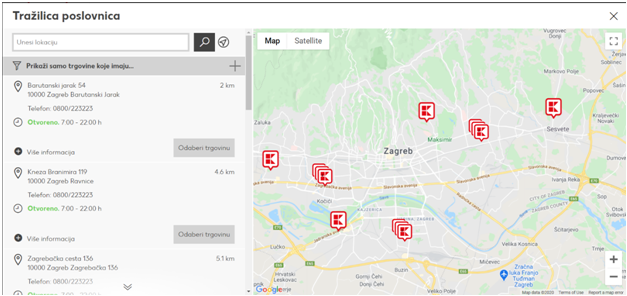
\includegraphics[scale=1]{slike/gmaps_p1.png} %veličina slike u odnosu na originalnu datoteku i pozicija slike
			\centering
			\caption{Odabir poslovnica tvrtke Kaufland,
				\url{https://www.kaufland.hr/usluge/poslovnica.html}
			}
			\label{fig:promjene}
		\end{figure}
	
				%unos slike
		\begin{figure}[H]
			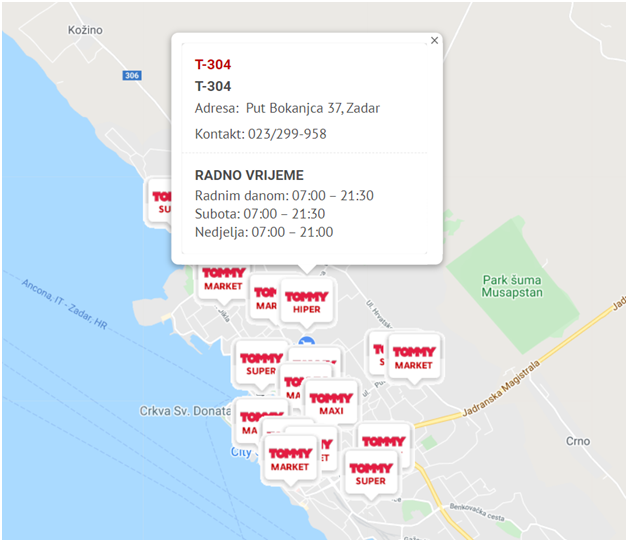
\includegraphics[scale=1]{slike/slika_2.png} %veličina slike u odnosu na originalnu datoteku i pozicija slike
			\centering
			\caption{Odabir poslovnica tvrtke Tommy,
				\url{ https://tommy.hr/hr/prodajna-mjesta}
			}
			\label{fig:promjene}
		\end{figure}

		
		\eject
		
	

	\chapter{Specifikacija programske potpore}
		
	\section{Funkcionalni zahtjevi}
			
			\noindent \textbf{Dionici:}
			
			\begin{packed_enum}
				
				\item Tvrtke	
				\item Korisnici
				
				\begin{packed_enum}
					

					\item Vozač
					
				\end{packed_enum}
				
				\item Administrator
				\item Razvojni tim
			
			\end{packed_enum}
			
			\noindent \textbf{Aktori i njihovi funkcionalni zahtjevi:}
			

			\begin{packed_enum}
				\item  \underbar{Tvrtka (inicijator) može:}
				
				\begin{packed_enum}
					
					\item registrirati se u aplikaciji unoseći OIB, ime, adresu sjedišta, adresu e-pošte 
					\item prijaviti, pregledati, urediti i obrisati parkirališnu površinu

				\end{packed_enum}
				
				\item  \underbar{Neregistrirani korisnik (inicijator) može:}
				
				\begin{packed_enum}
					
					\item pregledati parkirališne površine
					\item stvoriti korisnički račun unoseći OIB, ime, prezime, adresu e-ppošte, broj registracije svojeg automobila i broj kreditne kartice
					\item dobiti ovlasti registriranog korisnika
					
				\end{packed_enum}
				
				\item  \underbar{Vozač (inicijator) može:}
				
				\begin{packed_enum}
			
					\item pregledati parkirališne površine
					\item pregledati i promijeniti osobne podatke
					\item pregledati, dodati, obrisati registarsku oznaku automobila u aplikaciju
					\item dobiti prijedlog najbližih parkirališnih površina za rezervaciju
					\item rezervirati parkirališno mjesto
					\item platiti rezervaciju
					\item pregledati, urediti, obrisati rezervacije

				\end{packed_enum}

				\item  \underbar{Administrator (inicijator) može:}
				
				\begin{packed_enum}

					\item vidjeti popis odabranih korisnika
					\item urediti i obrisati odabrane korisnike
					\item vidjeti popis odabranih tvrtki
					\item urediti i obrisati odabrane tvrtke
						
				\end{packed_enum}
				
				\item  \underbar{Baza podataka (inicijator) može:}
				
				\begin{packed_enum}
					
					\item pohranjuje sve podatke o korisnicima
					\item pohranjuje sve podatke o tvrtkama
				
				\end{packed_enum}
			\end{packed_enum}
\eject 
				
			\subsection{Obrasci uporabe}
				
					\noindent \underbar{\textbf{UC1  - Pregled parkirališnih površina}}
					\begin{packed_item}
						
						\item  \textbf{Glavni sudionik: } Vozač, neregistrirani korisnik
						\item  \textbf{Cilj:} Pregledati parkirališne površine
						\item  \textbf{Sudionici:} Baza podataka, Google maps
						\item  \textbf{Preduvjet:} -
						\item  \textbf{Opis osnovnog tijeka:}
						
						\item[] \begin{packed_enum}
							\item Karta je prikazana prilikom otvaranja aplikacije
							\item Korisnik na karti odabire parkirališnu površinu
							\item Prikazuju se informacije o odabranoj površini
						\end{packed_enum}
						
					\end{packed_item}
					\noindent \underbar{\textbf{UC2  - Registracija}}
					\begin{packed_item}
						
						\item  \textbf{Glavni sudionik: } Neregistrirani korisnik, Tvrtka
						\item  \textbf{Cilj:} Stvoriti korisnički račun
						\item  \textbf{Sudionici:} Baza podataka
						\item  \textbf{Preduvjet:} -
						\item  \textbf{Opis osnovnog tijeka:}
						
						\item[] \begin{packed_enum}
							\item Korisnik odabire opciju za registraciju (vozač ili tvrtka)
							\item Korisnik unosi potrebne korisničke podatke
						\end{packed_enum}
						
						\item  \textbf{Opis mogućih odstupanja:}
						
						\item[] \begin{packed_item}
							
							\item[2.a]  Odabir već zauzetog korisničkog imena i/ili e-pošte, unos korisničkog podataka u nedozvoljenom formatu ili pružanje neispravne e-pošte
							\item[] \begin{packed_enum}
								
								\item Sustav obavještava korisnika o neuspjelom upisu i vraća ga na stranicu za registraciju
								\item Korisnik mijenja potrebne podatke te završava unos ili odustaje od registracije
								
							\end{packed_enum}
						\end{packed_item}
					\end{packed_item}
					\noindent \underbar{\textbf{UC3  - Prijava u sustav}}
					\begin{packed_item}
						
						\item  \textbf{Glavni sudionik: } Vozač
						\item  \textbf{Cilj:} Dobiti pristup korisničkom sučelju
						\item  \textbf{Sudionici:} Baza podataka
						\item  \textbf{Preduvjet:} Registracija
						\item  \textbf{Opis osnovnog tijeka:}
						
						\item[] \begin{packed_enum}
							\item Unos korisničkog imena i lozinke
							\item Potvrda ispravnosti unesenih podataka
							\item Pristup korisničkim funkcijama
						\end{packed_enum}
						
						\item  \textbf{Opis mogućih odstupanja:}
						
						\item[] \begin{packed_item}
							
							\item[2.a]  Neispravno uneseni podatci
								\item[] \begin{packed_enum}
								
									\item Sustav obavještava korisnika o neuspjeloj prijavi
								
								\end{packed_enum}
						\end{packed_item}
					\end{packed_item}
					\noindent \underbar{\textbf{UC4  - Pregled osobnih podataka}}
					\begin{packed_item}
						
						\item  \textbf{Glavni sudionik: } Vozač, Tvrtka
						\item  \textbf{Cilj:} Pregledati osobne podatke
						\item  \textbf{Sudionici:} Baza podataka
						\item  \textbf{Preduvjet:} Korisnik je prijavljen
						\item  \textbf{Opis osnovnog tijeka:}
						
						\item[] \begin{packed_enum}
							\item Korisnik odabire opciju „osobni podatci“
							\item Aplikacija prikazuje osobne podatke korisnika
						\end{packed_enum}
						
					\end{packed_item}
					\noindent \underbar{\textbf{UC5  - Promjena osobnih podataka}}
					\begin{packed_item}
						
						\item  \textbf{Glavni sudionik: } Vozač, tvrtka
						\item  \textbf{Cilj:} Promijeniti osobne podatke
						\item  \textbf{Sudionici:} Baza podataka
						\item  \textbf{Preduvjet:} Korisnik je prijavljen
						\item  \textbf{Opis osnovnog tijeka:}
						
						\item[] \begin{packed_enum}
							\item Korisnik odabire opciju „osobni podatci“
							\item Korisnik mijenja svoje osobne podatke
							\item Korisnik sprema promjene
							\item Baza podataka se ažurira
						\end{packed_enum}
						
						\item  \textbf{Opis mogućih odstupanja:}
						
						\item[] \begin{packed_item}
							
							\item[2.a]  Korisnik promijeni svoje osobne podatke, ali je nešto neispravno uneseno
							\item[] \begin{packed_enum}
								
								\item Sustav obavještava korisnika da je nemoguće izmjeniti podatke prilikom odabira „Spremi promjene“
								
							\end{packed_enum}
						\end{packed_item}
					\end{packed_item}
					\noindent \underbar{\textbf{UC6  - Registracija auta}}
					\begin{packed_item}
						
						\item  \textbf{Glavni sudionik: } Vozač
						\item  \textbf{Cilj:} Registrirati automobil
						\item  \textbf{Sudionici:} Baza podataka
						\item  \textbf{Preduvjet:} Vozač je prijavljen
						\item  \textbf{Opis osnovnog tijeka:}
						
						\item[] \begin{packed_enum}
							\item Vozač odabire opciju „dodaj auto“
							\item Vozač unosi potrebne podatke
							\item Vozač prima obavijest o uspješnoj registraciji
						\end{packed_enum}
						
						\item  \textbf{Opis mogućih odstupanja:}
						
						\item[] \begin{packed_item}
							
							\item[2.a]  Unesena neispravna/već registrirana registracija
							\item[] \begin{packed_enum}
								
								\item Sustav obavijesti vozača da nije moguće registrirati auto, te ga vraća na stranicu za registraciju automobila
								\item Vozač mijenja podatke ili odustaje
								
							\end{packed_enum}
						\end{packed_item}
					\end{packed_item}
					\noindent \underbar{\textbf{UC7  - Pregled registriranih automobila}}
					\begin{packed_item}
						
						\item  \textbf{Glavni sudionik: } Vozač
						\item  \textbf{Cilj:} Pregledati registrirane automobile
						\item  \textbf{Sudionici:} Baza podataka
						\item  \textbf{Preduvjet:} Vozač je prijavljen
						\item  \textbf{Opis osnovnog tijeka:}
						
						\item[] \begin{packed_enum}
							\item Vozač odabire opciju „pregledaj aute“
							\item Aplikacija prikazuje automobile koje je vozač prijašnje unio ako postoje
						\end{packed_enum}
						
					\end{packed_item}
					\noindent \underbar{\textbf{UC8  - Brisanje registriranih automobila}}
					\begin{packed_item}
						
						\item  \textbf{Glavni sudionik: } Vozač
						\item  \textbf{Cilj:} Obrisati registrirane automobile
						\item  \textbf{Sudionici:} Baza podataka
						\item  \textbf{Preduvjet:} Vozač je prijavljen
						\item  \textbf{Opis osnovnog tijeka:}
						
						\item[] \begin{packed_enum}
							\item Vozač odabere opciju „pregledaj aute“
							\item Vozač odabire auto koje želi obrisati i stisne  „obriši“
							\item Baza podataka se ažurira
						\end{packed_enum}
					\end{packed_item}
					\noindent \underbar{\textbf{UC9 - Rezervacija parkirališnog mjesta}}
					\begin{packed_item}
						
						\item  \textbf{Glavni sudionik: } Vozač
						\item  \textbf{Cilj:} Rezervirati parking mjesto
						\item  \textbf{Sudionici:} Baza podataka,  Google maps
						\item  \textbf{Preduvjet:} Vozač je prijavljen
						\item  \textbf{Opis osnovnog tijeka:}
						
						\item[] \begin{packed_enum}
							\item Vozač odabere opciju „Napravi rezervaciju“
							\item Sustav pronalazi vozaču najbližu parkirališnu površinu
							\item Vozač odabire ponuđenu parkirališnu površinu ili sam na karti pronalazi drugu
							\item Vozač odabire vozilo za koje želi napraviti rezervaciju
							\item Vozač ispuni potrebne informacije za rezervaciju
							\item Vozač odabire opciju „Potvrdi rezervaciju“
							\item Sustav naplati rezervaciju
						\end{packed_enum}
						
						\item  \textbf{Opis mogućih odstupanja:}
						
						\item[] \begin{packed_item}
							
							\item[3.a]  Na parkingu nema slobodnog mjesta
							\item[] \begin{packed_enum}
								
								\item Sustav obavještava vozača da nema slobodnog mjesta i daje korisniku opciju mijenjanja datuma rezervacije
								
							\end{packed_enum}
						\end{packed_item}
					\end{packed_item}
				
					\noindent \underbar{\textbf{UC10  - Pregled aktivnih rezervacija}}
					\begin{packed_item}
						
						\item  \textbf{Glavni sudionik: } Vozač
						\item  \textbf{Cilj:} Pregledati aktivne rezervacije
						\item  \textbf{Sudionici:} Baza podataka
						\item  \textbf{Preduvjet:} Vozač je prijavljen
						\item  \textbf{Opis osnovnog tijeka:}
						
						\item[] \begin{packed_enum}
							\item Vozač odabire opciju „Pregledaj rezervacije“
							\item Sustav prikaže vozaču aktivne rezervacije ukoliko takve postoje
						\end{packed_enum}
					
					\end{packed_item}
					
							
					\noindent \underbar{\textbf{UC11  - Brisanje aktivnih rezervacija}}
					\begin{packed_item}
						
						\item  \textbf{Glavni sudionik: } Vozač
						\item  \textbf{Cilj:} Obrisati rezervaciju
						\item  \textbf{Sudionici:} Baza podataka
						\item  \textbf{Preduvjet:} Vozač je prijavljen i napravio je barem jednu rezervaciju
						\item  \textbf{Opis osnovnog tijeka:}
						
						\item[] \begin{packed_enum}
							\item Vozač odabire opciju „Pregledaj rezervacije“
							\item Sustav prikaže listu rezervacija vozača
							\item Vozač odabire opciju „Obriši rezervaciju“
							\item Rezervacija se briše iz baze podataka
							\item Vozaču se vraćaju novci ako ima neiskorištenih rezervacija
						\end{packed_enum}
						
						\item  \textbf{Opis mogućih odstupanja:}
						
						\item[] \begin{packed_item}
							
							\item[4.a]  Greška prilikom refundiranja novca
							\item[] \begin{packed_enum}
								
								\item Sustav obavještava vozača da je došlo do greške prilikom refundiranja novca na njegov račun, te se odustaje od brisanja rezervacije.
								
							\end{packed_enum}
						\end{packed_item}
						
					\end{packed_item}
					\noindent \underbar{\textbf{UC12 - Prijava parkirališne površine}}
					\begin{packed_item}
						
						\item  \textbf{Glavni sudionik: } Tvrtka
						\item  \textbf{Cilj:} Prijaviti parking objekt
						\item  \textbf{Sudionici:} Baza podataka
						\item  \textbf{Preduvjet:} Tvrtka je prijavljena
						\item  \textbf{Opis osnovnog tijeka:}
						
						\item[] \begin{packed_enum}
							\item Tvrtka odabire opciju „Dodaj parkirališnu površinu“
							\item Unos podataka o parkirališnoj površini
							\item Tvrtka unese sve podatke i odabire „Spremi“
							\item Ažurira se baza podataka
						\end{packed_enum}
						
						\item  \textbf{Opis mogućih odstupanja:}
						
						\item[] \begin{packed_item}
							
							\item[2.a]  Unesen neispravan/već prijavljen parking
							\item[] \begin{packed_enum}
								
								\item Sustav obavijesti korisnika da nije moguće prijaviti parking te ga vraća na stranicu za prijavu parkirališne površine
								\item Korisnik mijenja podatka ili odustaje
								
							\end{packed_enum}
						\end{packed_item}
					\end{packed_item}
					\noindent \underbar{\textbf{UC13  - Pregled prijavljenih parkirališnih površina}}
					\begin{packed_item}
						
						\item  \textbf{Glavni sudionik: } Tvrtka
						\item  \textbf{Cilj:} Pregled prijavljenih parkirališnih površina
						\item  \textbf{Sudionici:} Baza podataka
						\item  \textbf{Preduvjet:} Tvrtka je prijavljena i postoji prijavljena parkirališna površina
						\item  \textbf{Opis osnovnog tijeka:}
						
						\item[] \begin{packed_enum}
							\item Korisnik odabire opciju „Upravljaj parkirališnim površinama“
							\item Otvara se lista prijavljenih parkirališnih površina
						\end{packed_enum}
						
					\end{packed_item}
					
					\noindent \underbar{\textbf{UC14  - Brisanje parkirališnih površina}}
					\begin{packed_item}
						
						\item  \textbf{Glavni sudionik: } Tvrtka
						\item  \textbf{Cilj:} Obrisati parkirališnu površinu
						\item  \textbf{Sudionici:} Baza podataka
						\item  \textbf{Preduvjet:} - Tvrtka je prijavljena i ima barem jedan prijavljeni parkirališnu površinu
						\item  \textbf{Opis osnovnog tijeka:}
						
						\item[] \begin{packed_enum}
							\item Korisnik odabire opciju „Upravljaj parkirališnim površinama“
							\item Sustav prikaže listu prijavljenih parkirališnih površina
							\item Korisnik briše željenu parkirališnu površinu
							\item Ažurira se baza podataka

						\end{packed_enum}
						
					\end{packed_item}
					\noindent \underbar{\textbf{UC15  - Pregled vozača}}
					\begin{packed_item}
						
						\item  \textbf{Glavni sudionik: }Administrator
						\item  \textbf{Cilj:}  Vidjeti popis vozača
						\item  \textbf{Sudionici:} Baza podataka
						\item  \textbf{Preduvjet:} - Administrator prijavljen
						\item  \textbf{Opis osnovnog tijeka:}
						
						\item[] \begin{packed_enum}
							\item Administrator odabire opciju „Popis vozača“
							\item Pojavi se lista vozača
						\end{packed_enum}
						
					\end{packed_item}
					\noindent \underbar{\textbf{UC16  - Uređivanje vozača}}
					\begin{packed_item}
						
						\item  \textbf{Glavni sudionik: } Administrator
						\item  \textbf{Cilj:} Urediti vozače
						\item  \textbf{Sudionici:} Baza podataka
						\item  \textbf{Preduvjet:} Administrator prijavljen i postoji barem jedan korisnik
						\item  \textbf{Opis osnovnog tijeka:}
						
						\item[] \begin{packed_enum}
							\item Administrator pronalazi željenog vozača i odabire opciju „Uredi“
							\item Sustav prikazuje podatke o odabranom vozaču
							\item Administrator upravlja njegovim podacima
							\item Ažurira se baza podataka
						\end{packed_enum}
						
					\end{packed_item}
					\noindent \underbar{\textbf{UC17  - Brisanje vozača}}
					\begin{packed_item}
						
						\item  \textbf{Glavni sudionik: } Admin
						\item  \textbf{Cilj:}  sudionik: Obrisati odabranog vozača
						\item  \textbf{Sudionici:} Baza podataka
						\item  \textbf{Preduvjet:} Admin prijavljen i postoji barem jedan korisnik
						\item  \textbf{Opis osnovnog tijeka:}
						
						\item[] \begin{packed_enum}
							\item Administrator pronalazi željenog vozača i odabire opciju „Obriši“
							\item Vozač se obriše
							\item Ažurira se baza podataka
						\end{packed_enum}
						
					\end{packed_item}
					\noindent \underbar{\textbf{UC18  - Pregled tvrtki}}
					\begin{packed_item}
						
						\item  \textbf{Glavni sudionik: } Admin
						\item  \textbf{Cilj:} Vidjeti popis odabranih tvrtki
						\item  \textbf{Sudionici:} Baza podataka
						\item  \textbf{Preduvjet:} Admin prijavljen
						\item  \textbf{Opis osnovnog tijeka:}
						
						\item[] \begin{packed_enum}
							\item Administrator odabire opciju „Popis tvrtki“
							\item Pojavi se lista s odabranim tvrtkama
						\end{packed_enum}
						
					\end{packed_item}
					\noindent \underbar{\textbf{UC19  - Uređivanje odabranih tvrtki}}
					\begin{packed_item}
						
						\item  \textbf{Glavni sudionik: } Administrator
						\item  \textbf{Cilj:} Urediti odabrane tvrtke
						\item  \textbf{Sudionici:} Baza podataka
						\item  \textbf{Preduvjet:} Administrator prijavljen i postoji barem jedna tvrtka
						\item  \textbf{Opis osnovnog tijeka:}
						
						\item[] \begin{packed_enum}
							\item Administrator pronalazi željenu tvrtku i odabire opciju „Uredi“
							\item Sustav prikazuje podatke o odabranoj tvrtki
							\item Administrator upravlja njezinim podacima
							\item Ažurira se baza podataka
						\end{packed_enum}
						
					\end{packed_item}
					\noindent \underbar{\textbf{UC20  - Brisanje odabranih tvrtki}}
					\begin{packed_item}
						
						\item  \textbf{Glavni sudionik: } Administrator
						\item  \textbf{Cilj:} Obrisati odabrane tvrtke
						\item  \textbf{Sudionici:} Baza podataka
						\item  \textbf{Preduvjet:} - Administrator je prijavljen i postoji barem jedan korisnik
						\item  \textbf{Opis osnovnog tijeka:}
						
						\item[]	\begin{packed_enum}
							\item Administrator odabire željenu tvrtku i odabire opciju „Obriši“
							\item Tvrtka se obriše
							\item Ažurira se baza podataka
						\end{packed_enum}
					
					\end{packed_item}
							
			\eject		
			
				\subsubsection{Dijagrami obrazaca uporabe}
				
					%unos slike
					\begin{figure}[H]
						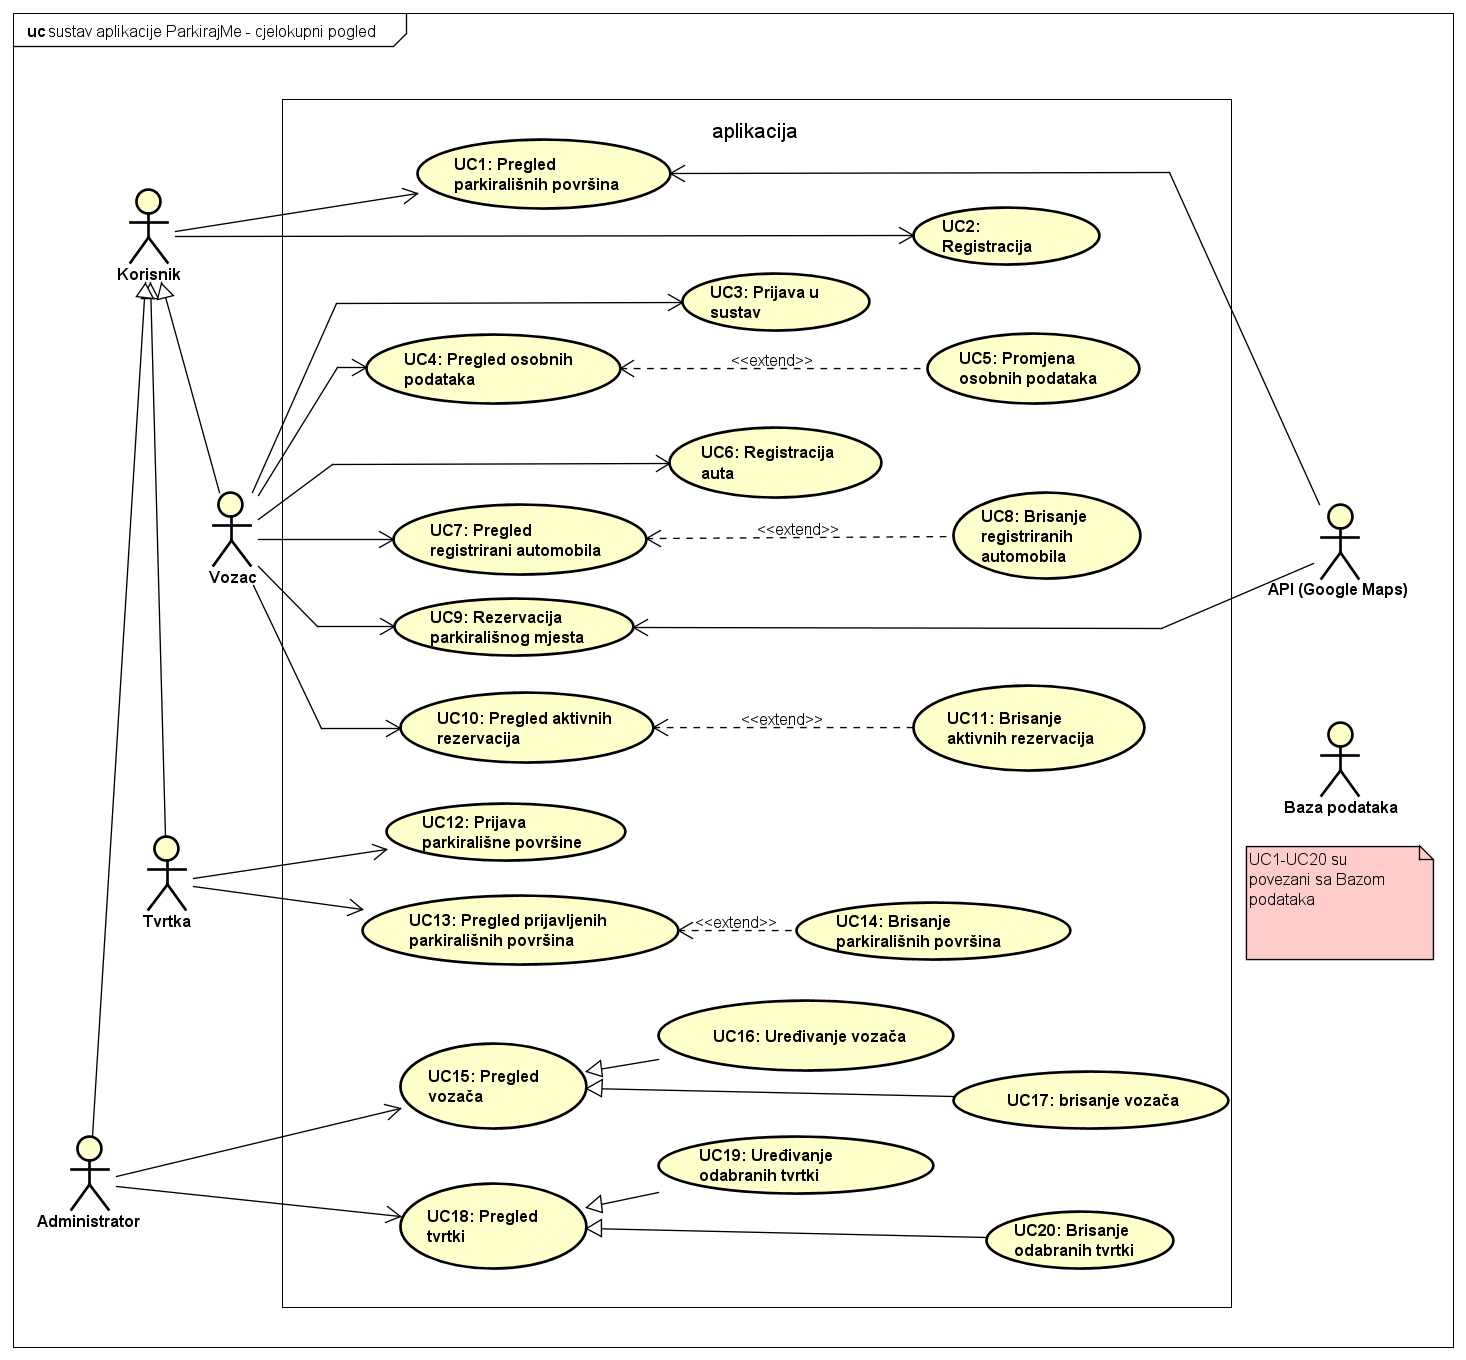
\includegraphics[scale=0.4]{dijagrami/cjelokupni_pogled.png} %veličina slike u odnosu na originalnu datoteku i pozicija slike
						\centering
						\caption{Cjelokupni pogled}
						\label{fig:promjene}
					\end{figure}
				
					%unos slike
					\begin{figure}[H]
						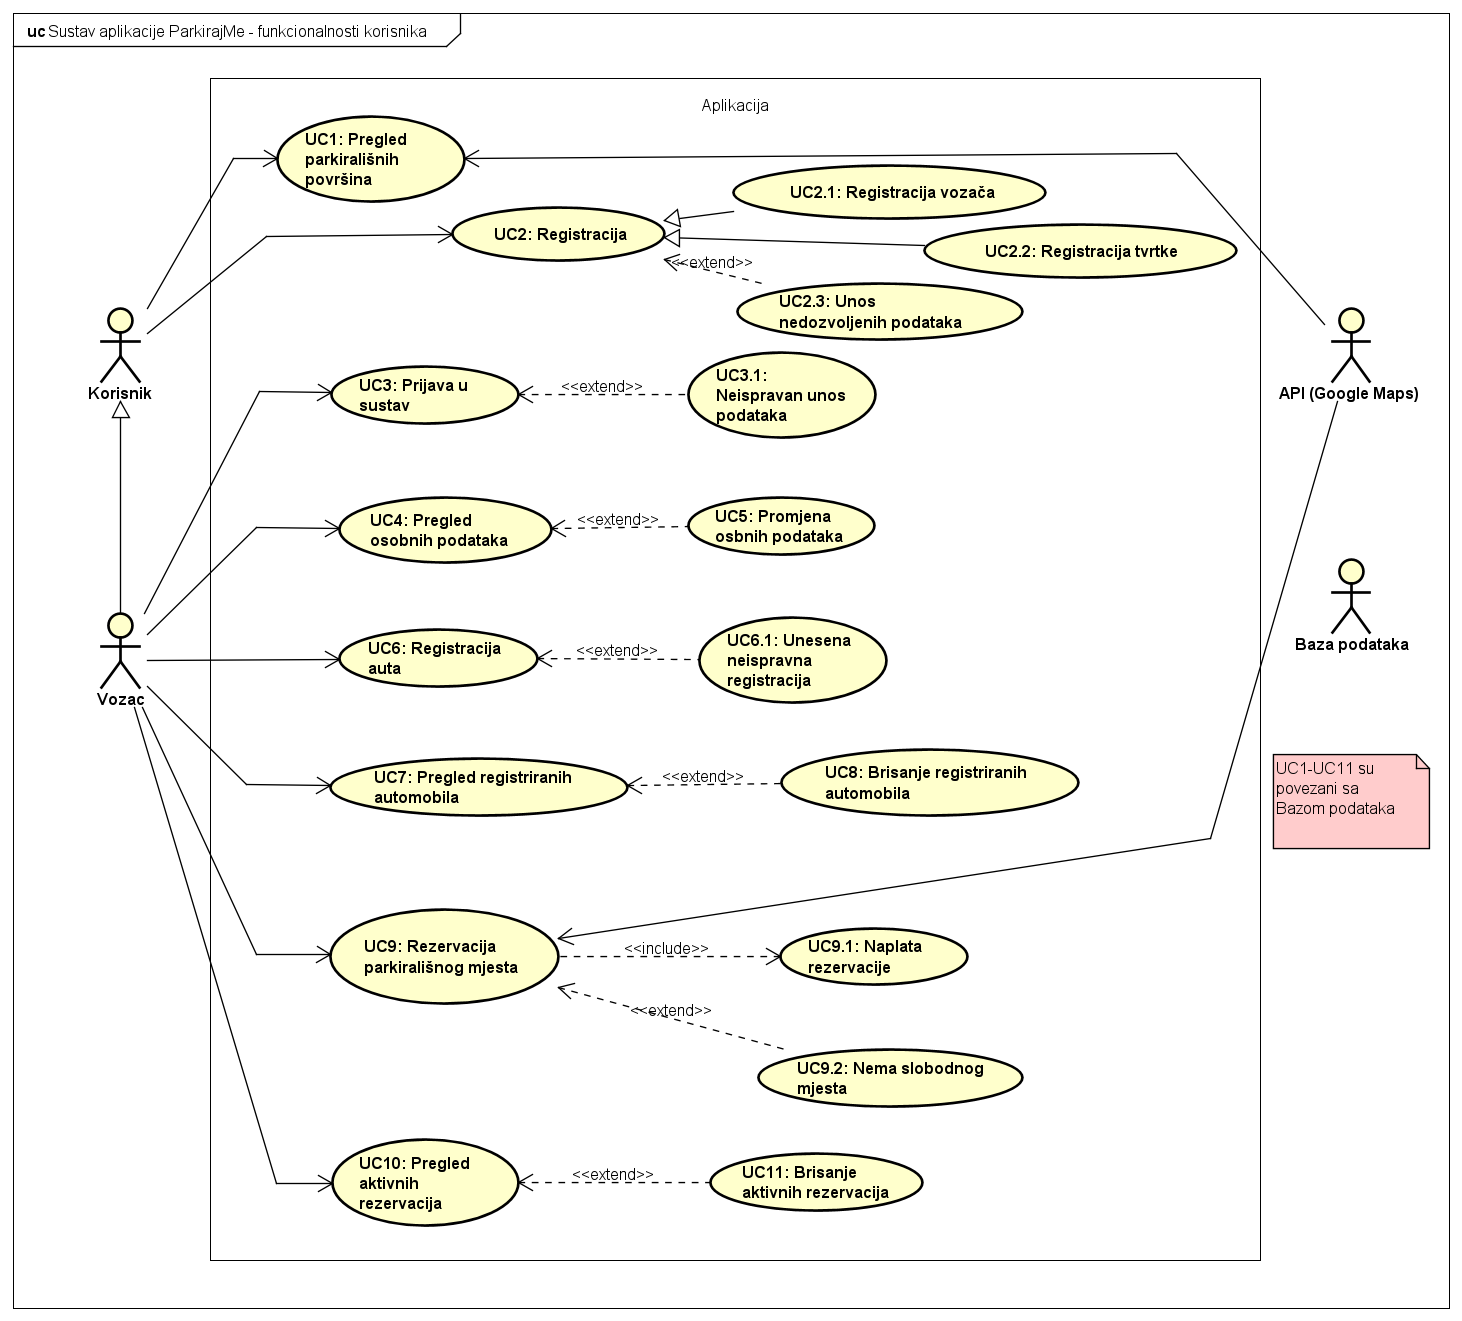
\includegraphics[scale=0.4]{dijagrami/funkcionalnosti_korisnika.png} %veličina slike u odnosu na originalnu datoteku i pozicija slike
						\centering
						\caption{Funkcionalnosti korisnika}
						\label{fig:promjene}
					\end{figure}
				
					%unos slike
					\begin{figure}[H]
						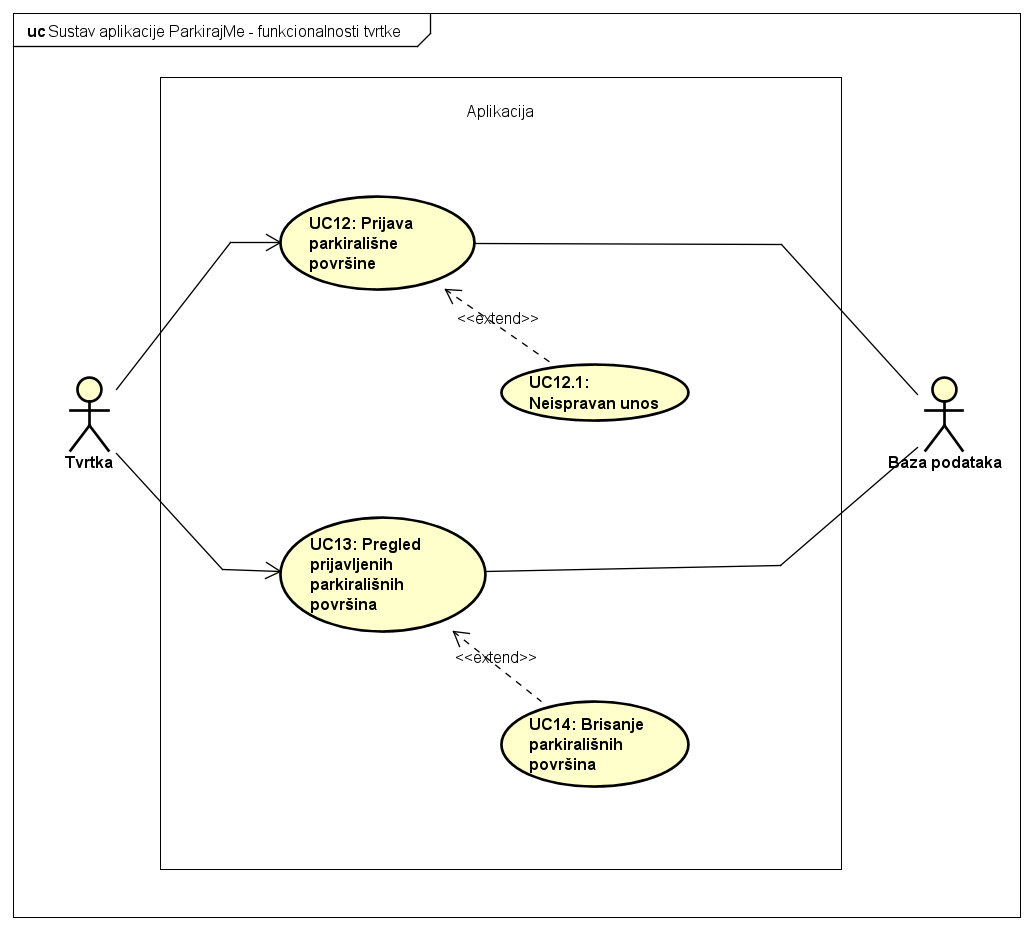
\includegraphics[scale=0.55]{dijagrami/funkcionalnosti_tvrtke.png} %veličina slike u odnosu na originalnu datoteku i pozicija slike
						\centering
						\caption{Funkcionalnosti tvrtke}
						\label{fig:promjene}
					\end{figure}
				
					%unos slike
					\begin{figure}[H]
						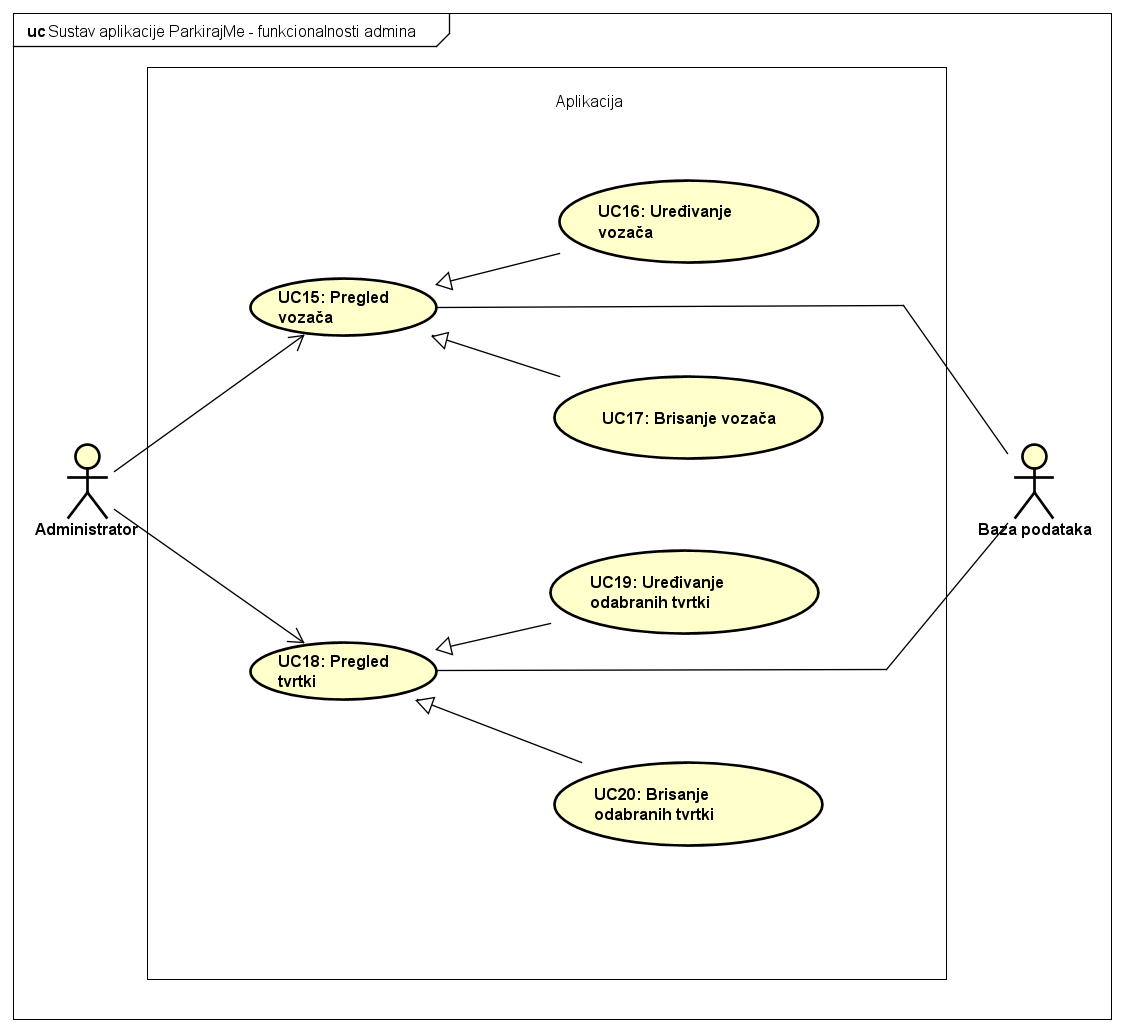
\includegraphics[scale=0.5]{dijagrami/funkcionalnosti_admina.png} %veličina slike u odnosu na originalnu datoteku i pozicija slike
						\centering
						\caption{Funkcionalnosti admina}
						\label{fig:promjene}
					\end{figure}				
				\eject		
				
			\subsection{Sekvencijski dijagrami}
				
				
				\noindent {\textbf{Obrazac uporabe UC2 - Registracija}}\\
				Korisnik bira jednu od dvije opcije registracije: "Registriraj se kao korisnik" ili "Registriraj se kao tvrtka". Nakon odabira željene registracije aplikacija ga traži unos potrebnih podataka. Aplikacija provjerava jesu li sva polja popunjena i je li format unesenih podataka ispravan (broj znamenki OIB-a,format adrese e-pošte...). Nakon toga aplikacija pristupa bazi podataka i provjerava jedinstvenost unesenih podataka. Ako su podaci ispravni, ovisno o vrsti registracije, stvara se novi vozač ili korisnički račun tvrtke te se podaci pohranjuju u bazu podataka. Ako su uneseni podaci neispravni, korisnik prima obavijest i aplikacija ga vraća na glavni izbornik.
	

				\begin{figure}[H]
					\includegraphics[scale=0.5]{dijagrami/Sekvencijski dijagram - Registracija.png} %veličina slike u odnosu na originalnu datoteku i pozicija slike
					\centering
					\caption{Sekvencijski dijagram - Registracija}
					\label{fig:promjene}
				\end{figure}	
			
				\newpage
				\noindent {\textbf{Obrazac uporabe UC11 - Brisanje aktivnih rezervacija}}\\
				Vozač odabire opciju "pregledaj rezervacije" nakon čega poslužitelj pristupa bazi podataka i dohvaća listu svih vozačevih rezervacija. Vozač odabire jednu rezervaciju koju želi obrisati i klikom na gumb "obriši" rezervacije se briše. Ako rezervacija još nije iskorištena, aplikacija uplaćuje cijenu rezervacije na vozačev račun i briše ju iz baze podatatka. Ako je rezervacija već iskorištena, aplikacija ju uklanja iz baze podataka. Nakon brisanja rezervacije, korisnik se vraća na glavni izbornik.
			\\
				
				\begin{figure}[H]
					\includegraphics[scale=0.5]{dijagrami/Sekvencijski dijagram -brisanje aktivnih rezervacija.png} %veličina slike u odnosu na originalnu datoteku i pozicija slike
					\centering
					\caption{Sekvencijski dijagram - Brisanje aktivnih rezervacija}
					\label{fig:promjene}
				\end{figure}	
			
				\newpage
			\noindent {\textbf{Obrazac uporabe UC12 - Prijava parkirališne površine}}\\
			Korisnik koji je prijavljen sa korisničkim računom tvrtke može prijaviti novu parkirališnu površinu. Odabirom opcije "Dodaj parkirališnu površinu" otvara se izbornik koji od korisnika traži unos podataka. Klikom miša na karti, korisnik postavlja marker na željenu lokaciju i time označava mjesto parkirališne površine. Google Karte prosljeđuju koordinate lokacije aplikaciji te aplikacija prikazuje koordinate korisniku. Ako korisnik nije zadovoljan odabranim koordinatama, klikom na opciju "restartaj marker" može ponovno označiti lokaciju na karti. Nakon što korisnik unese ostale tražene podatke i odabere "spremi lokaciju", podaci se spremaju u bazu podataka.
			
			\begin{figure}[H]
				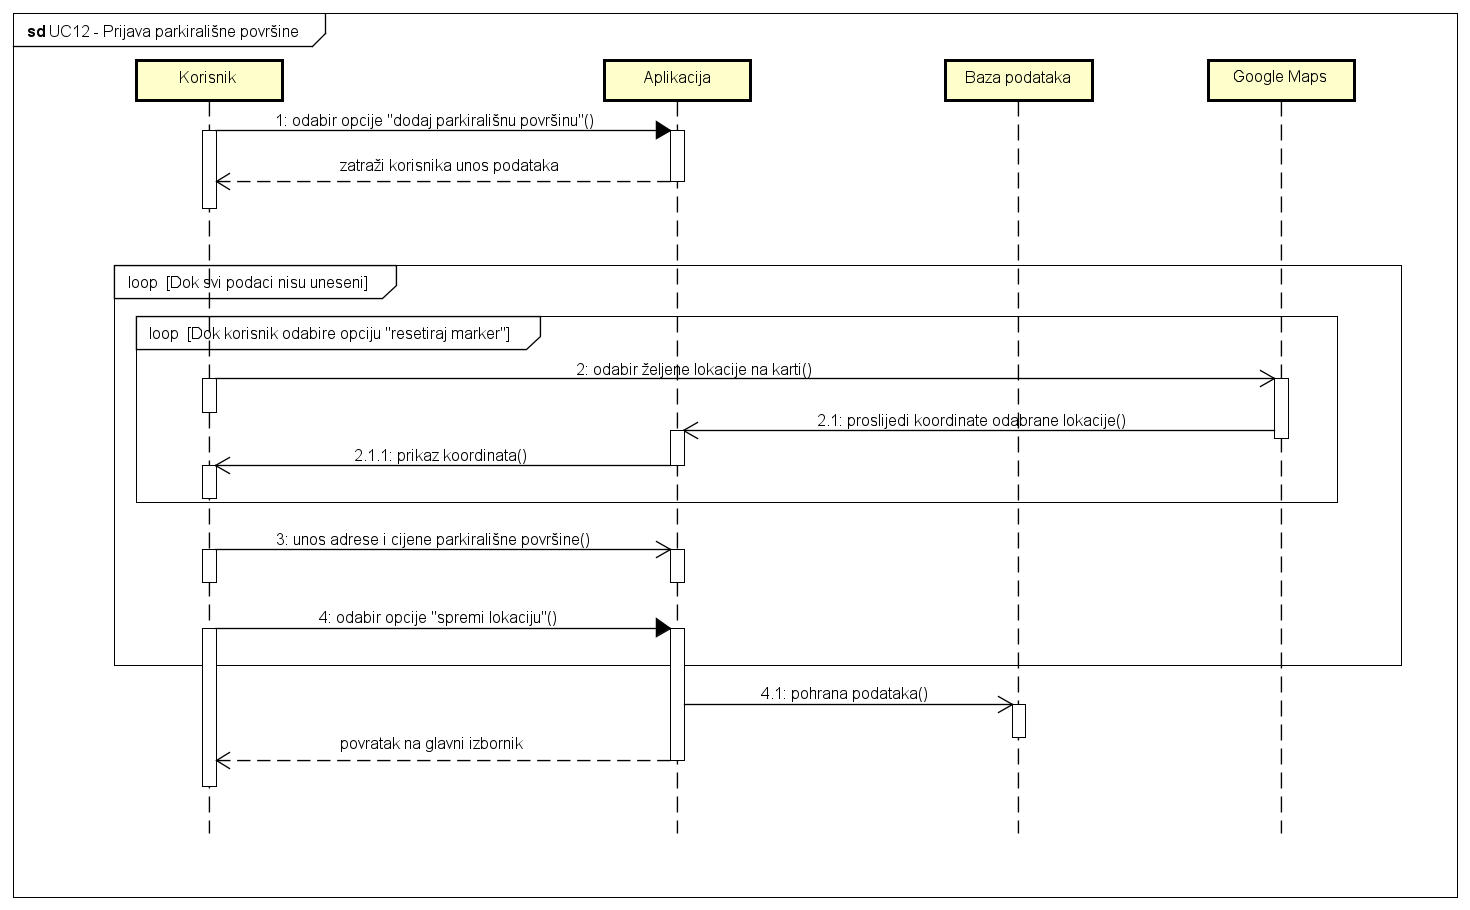
\includegraphics[scale=0.4]{dijagrami/sekvencijski dijagram - prijava parkirališne površine.png} %veličina slike u odnosu na originalnu datoteku i pozicija slike
				\centering
				\caption{Sekvencijski dijagram - prijava parkirališne površine}
				\label{fig:promjene}
			\end{figure}
			
				\newpage
				\noindent {\textbf{Obrazac uporabe UC17 - Brisanje vozača}}\\
				Administrator može pregledati i upravljati svim vozačima. Odabirom opcije "Popis vozača" prikazuje se lista svih prijavljenih vozača. Klikom na gumb "Obriši" pored željenog vozača, aplikacija pristupa bazi podataka i uklanja ga. Baza podataka šalje novi popis prijavljenih vozača, aplikacija se ažurira i prikazuje novu listu svih vozača.
			 \\
		
				\begin{figure}[H]
					\includegraphics[scale=0.5]{dijagrami/Sekvencijski dijagram - brisanje vozača.png} %veličina slike u odnosu na originalnu datoteku i pozicija slike
					\centering
					\caption{Sekvencijski dijagram - brisanje vozača}
					\label{fig:promjene}
				\end{figure}		
				
				\eject
	
		\section{Ostali zahtjevi}
			 
			 \begin{packed_item}
			 	
			 	\item  Sustav treba omogućiti rad više korisnika u stvarnom vremenu 
			 	\item  Sustav mora podržavati hrvatsku abecedu koji se mogu pojavljivati u korisničkim imenima i nazivima objekata na karti grada Zagreba
			 	\item  Komunikacija sa bazom podataka (slanje upita i primanje odgovora od baze) ne smije trajati dulje od nekoliko sekundi
			 	\item  Sustav treba biti implementiran kao web aplikacija
			 	\item  Korištenje sustava na način na koji nije zamišljeno ne smije narušiti funkcionalnost i rad
			 	\item  Sustav treba biti intuitivan za korištenje
			 	\item  Nadogradnja sustava provodi se na temelju zadnje verzije bez mijenjanja ključnih dijelova sustava
			 	\item Sustav kao valutu treba podržati HRK
			 	\item Cijene rezervacija prikazuju točan iznos do drugog decimalnog mjesta
			 	\item Baza podataka treba biti otporna na napade i greške
			 	\item Pristup sustavu treba biti omogućen iz javne mreže pomoću HTTPS-a
			 	\item Sustav korisniku mora omogućiti registraciju neograničenog broja automobila
			 	\item Lokacija parkirališnih površina ima odstupanje od maksimalno 30 metara
			 	\item Sustav je dostupan 24 sata dnevno, 365 dana u godini (osim u trenucima obnavljanja ili nadogradnje sustava)
			 	
			 \end{packed_item}
			 
	
	
	\chapter{Arhitektura i dizajn sustava}

		\textit{Arhitektura je podjeljena na tri sustava:}
	\begin{itemize}
		\item 	\textit{Web Aplikacija}
		\item 	\textit{Web Poslužitelj}
		\item 	\textit{Baze podataka}		
	\end{itemize}
	
	%unos slike
			\begin{figure}[H]
				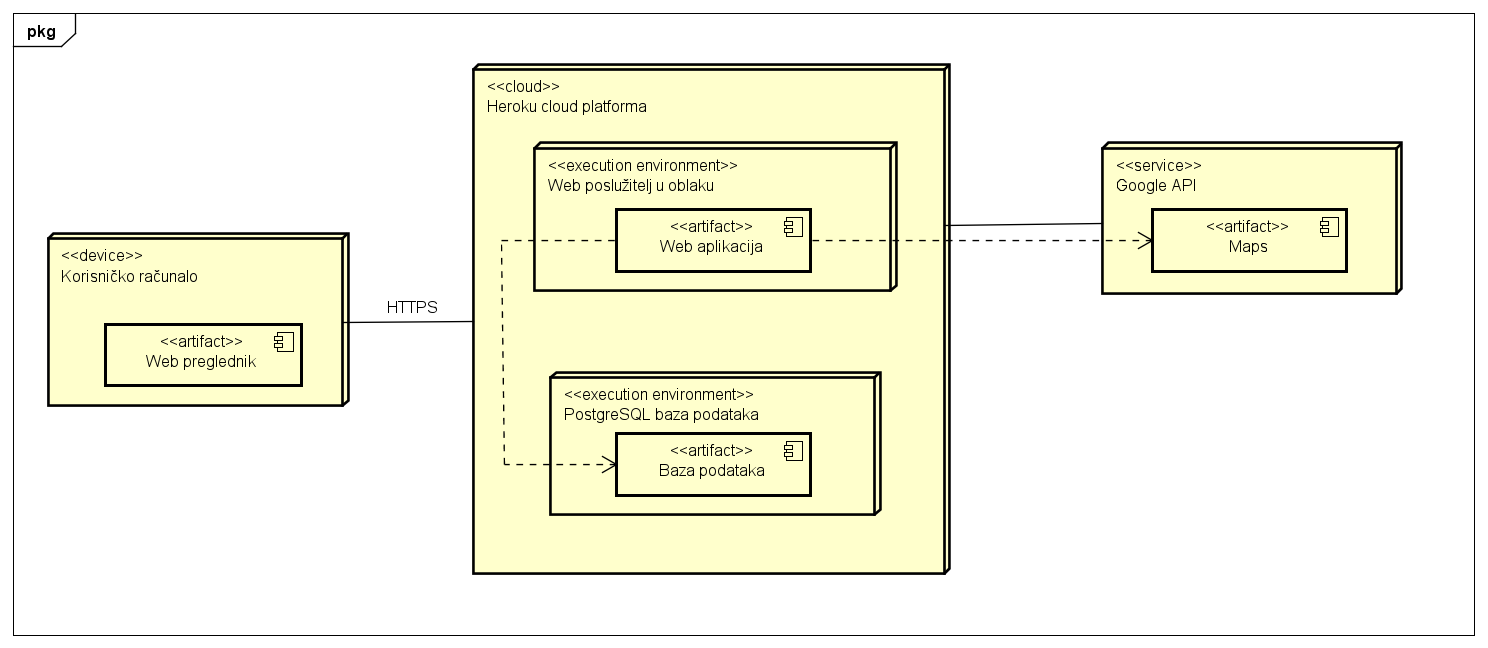
\includegraphics[scale=0.4]{dijagrami/dijagram_razmjestaja.png} %veličina slike u odnosu na originalnu datoteku i pozicija slike
				\centering
				\caption{Dijagram arhitekture sustava}
				\label{fig:promjene}
			\end{figure}

		Korisnik aplikaciji pristupa preko web preglednika. \textit{Web preglednik} je program kojim korisnik pristupa web sadržaju. Jedna od njegovih glavnih zadaća je prevođenje koda u konačni produkt sa svim sadržajima namijenjen korisniku. 
		
		Pošto je aplikacija dinamička, preglednik komunicira s web aplikacijom preko \textit{web poslužitelja}, odnosno servera, čija je glavna zadaća prosljeđivanje korisničkih zahtjeva aplikaciji. Ta komunikacija odvija se preko HTTPS protokola kako bi se omogućio siguran prijenos korisnikovih podataka i informacija.
		
		\textit{Web aplikacija} obrađuje te zahtjeve, pristupa bazi podatka i ostalim vanjskim servisima po potrebi te šalje odgovor na korisinkov zahtjev u obliku HTML dokumenta razmuljiv web pregledniku. Ako se zahtjev nije uspio izvršiti, aplikacija će korinsiku dojaviti pogrešku. 
		
		\textit{Baza podataka} služi za pohranu, izmjenu i dohvat podataka koji će se obrađivati u aplikaciji. Za njenu implementaciju koristiti ćemo Postgresql.
	
		Za izradu web aplikacije odlučili smo koristiti Node.js, te ćemo većinu funkcionalnosti aplikacije ostvariti uz pomoć Express frameworka te Pug HTML template enginea. Za spajanje aplikacije s bazom podataka koristiti ćemo Connect-pg-Simple.
		
			Aplikaciju ćemo razvijati
		u razvojnom okruženju Microsoft Visual Studio. 
			Arhitektura sustava temeljit će se na 
		Model-View-Controller (MVC) arhitekturi. 
		
		
		\newpage
				
		\section{Baza podataka}
			
			Za naš sustav koristiti ćemo relacijsku bazu podataka, ostvarenu u aplikaciji Postgresql. Baza je prilagođena brzom pohranjivanju i dohvaćanju podataka, te su entiteti napravljeni tako da odgovaraju modelima u dijagramu razreda.
			
				Baza podataka sastoji se od sljedećih entiteta:
				\begin{itemize}
					\item 	\textit{Korisnik}
					\item 	\textit{Tvrtka}
					\item 	\textit{Parking}
					\item 	\textit{Vozilo}
					%		\item 	\textit{Vozi}
					\item 	\textit{Rezervacija}
					\item 	\textit{Sjednica}
				\end{itemize}
		
			\subsection{Opis tablica}
			

				
				\textbf{Korisnik}  je entitet koji čuva informacije o korisniku aplikacije \textit{ParkirajMe}. Sadrži atribute: Korisničko ime i OIB korisnika, broj kreditne kartice, e-mail korisnika, te njegovo ime i prezime. Ovaj entitet u vezi je \textit{One-to-Many} s entitetom vozilo preko korisničkog imena, zato jer svaki korisnik može posjedovati više vozila, a jedno vozilo također može imati više korisnika koji ga parkiraju.
				


				\begin{longtabu} to \textwidth {|X[10, l]|X[6, l]|X[20, l]|}
					
					\hline \multicolumn{3}{|c|}{\textbf{korisnik}}	 \\[3pt] \hline
					\endfirsthead
					
					\hline \multicolumn{3}{|c|}{\textbf{korisnik}}	 \\[3pt] \hline
					\endhead
					
					\hline 
					\endlastfoot
					

					Korisničko ime	& VARCHAR &		Jedinstveno korisničko ime korisnika   	\\ \hline 
					Lozinka	& VARCHAR &		Hash jedinstvene lozinke korisnika   	\\ \hline 
					OIB & CHAR(11)	&  	Osobni identifikacijski broj korisnika 	\\ \hline
					Broj kred. kartice	& VARCHAR &   	Broj kreditne kartice korisnika	\\ \hline 
					Email & VARCHAR & 		adresa elektroničke pošte korisnika  \\ \hline 
					Ime & VARCHAR	&  		Ime korisnika	\\ \hline 
					Prezime	& VARCHAR &		Prezime korisnika   	\\ \hline 
					Razina ovlasti	& INT &		Razina ovlasti korisnika   	\\ \hline 
					
					
				\end{longtabu}
			
			\textbf{Tvrtka} je entitet koji predstavlja korisnički račun tvrtke koji je u njeno ime otvorio ovlašteni zaposlenik tvrtke. Sadrži atribute: korisničko ime, lozinka, OIB tvrtke, Email , ime te adresu sjedišta. Povezan je vezom \textit{One-To-Many} s entitetom parking, zato jer je jedna tvrtka može imati više parkinga.
			
			
				\begin{longtabu} to \textwidth {|X[10, l]|X[6, l]|X[20, l]|}
				
				\hline \multicolumn{3}{|c|}{\textbf{tvrtka}}	 \\[3pt] \hline
				\endfirsthead
				
				\hline \multicolumn{3}{|c|}{\textbf{tvrtka}}	 \\[3pt] \hline
				\endhead
				
				\hline 
				\endlastfoot
				
				\cellcolor{green}Korisničko ime	& VARCHAR &		Jedinstveno korisničko ime ovlaštenog zaposlenika tvrtke   	\\ \hline 
				Lozinka	& VARCHAR &		Hash jedinstvene lozinke ovlaštenog zaposlenika tvrtke   	\\ \hline 
				OIB tvrtke & CHAR(11)	&  	Osobni identifikacijski broj tvrtke 	\\ \hline
				Email & VARCHAR & 		adresa elektroničke pošte tvrtke  \\ \hline 
				Ime & VARCHAR	&  		Ime tvrtke	\\ \hline 
				\cellcolor{LightBlue} adresaTvrtka	& VARCHAR &		Adresa sjedišta tvrtke   	\\ \hline 
				
				
			\end{longtabu}
		
		\textbf{Vozilo} je entitet koji pohranjuje koja sve vozila je u aplikaciju unio neki korisnik, te su to jedina dva atributa ovog entiteta. U vezi je \textit{Many-to-One} s entitetom korisnik preko atributa korisničko ime, te u vezi \textit{One-to-Many}  s entitetom rezervacija preko atributa registracija.
		
			\begin{longtabu} to \textwidth {|X[10, l]|X[6, l]|X[20, l]|}
				
				\hline \multicolumn{3}{|c|}{\textbf{vozilo}}	 \\[3pt] \hline
				\endfirsthead
				
				\hline \multicolumn{3}{|c|}{\textbf{ozilo}}	 \\[3pt] \hline
				\endhead
				
				\hline 
				\endlastfoot
				
				Korisničko ime	& VARCHAR &		Jedinstveno korisničko ime vlasnika vozila   	\\ \hline 
				Registracija	& VARCHAR &		Registracija automobila   	\\ \hline 
			 
				
				
				
			\end{longtabu}
		
		\textbf{Rezervacija} je entitet koji sadržava podatke o rezervaciji jednog parkirnog mjesta. Njezini atributi su: ID rezervacije, ID grupe rezervacija kojoj ova rezervacija pripada,  Korisničko ime onog tko je rezervirao, registracija vozila, ID parkinga, datum i vrijeme početka i kraja rezervacije. Povezan je vezom \textit{Many-to-One} sa entitetom Vozilo preko atributa Korisničko ime i rezervacija (Ključ entiteta vozilo), te s entitetom Parking vezom \textit{Many-to-One} preko atributa Parking ID.
			
			\begin{longtabu} to \textwidth {|X[10, l]|X[6, l]|X[20, l]|}
				
				\hline \multicolumn{3}{|c|}{\textbf{rezervacija}}	 \\[3pt] \hline
				\endfirsthead
				
			%	\hline \multicolumn{3}{|c|}{\textbf{rezervacija}}	 \\[3pt] \hline
			%	\endhead
				
			%	\hline 
				\endlastfoot
				
				\cellcolor{green}IDRezervacija	& SERIAL &		Jedinstveni ID rezervacije  	\\ \hline 
				ID grupe	& INT &		Jedinstvena oznaka grupe rezervacija  	\\ \hline
				Korisničko ime	& VARCHAR &		Jedinstveno korisničko ime vlasnika vozila   	\\ \hline
				Registracija vozila	& VARCHAR &		Registracija automobila koji će zauzeti mjesto   	\\ \hline 
				IDParking	& INT &		Jedinstvena oznaka parkinga  	\\ \hline 
				Pocetak rezervacije & TIMESTAMP	&  	Početak rezervacije 	\\ \hline
				Kraj rezervacije & TIMESTAMP & 		Završetak rezervacije  \\ \hline 
				
				
				
			\end{longtabu}
		
		\textbf{Parking} je entitet koji sadržava podatke o jednom parkingu. Njegovi atributi su: ID parkinga, OIB tvrtke koja ga je objavila, ukupan kapacitet, broj slobodnih mjesta, cijena parkirnog mjesta, adresa parkinga, te geografska širina i dužina njegove lokacije. Povezan je sa entitetom tvrtka vezom \textit{Many-to-One} pošto jedna tvrtka može imati više parkinga, te s entitetom rezervacije vezom \textit{One-to-Many} zato jer na jednom parkingu može biti više rezervacija. Također je povezan s entitetom Lokacija vezom \textit{One-to-One} preko atributa ID lokacija.
		
		\begin{longtabu} to \textwidth {|X[10, l]|X[6, l]|X[20, l]|}
			
			\hline \multicolumn{3}{|c|}{\textbf{parking}}	 \\[3pt] \hline
			\endfirsthead
			
			\hline \multicolumn{3}{|c|}{\textbf{parking}}	 \\[3pt] \hline
			\endhead
			
			\hline 
			\endlastfoot
			
			
			ID parkinga	& SERIAL &		Jedinstvena oznaka parkinga   	\\ \hline
			Korisničko ime tvrtke	& VARCHAR & korisničko	ime tvrtke koja je vlasnik parkinga  	\\ \hline 
			Kapacitet	& INT &		Ukupan kapacitet parkinga 	\\ \hline 
			Broj slob. mjesta & INT	&  	Broj slobodnih mjesta na parkingu 	\\ \hline
			Cijena po satu & NUMERIC & 		Cijena rezervacije parkinga po satu  \\ \hline 
			ID lokacija	& INT & Jedinstvena oznaka lokacije parkinga 	\\ \hline
			
		\end{longtabu}
	
		
		
			\textbf{Lokacija} je entitet koji sadržava podatke o jednoj lokaciji. Njegovi atributi su ID lokacije, njena adresa,  te geografska širina i dužina. Povezan je vezom \textit{One-to-One} s entitetom Parking zato jer se na jednoj lokaciji može nalaziti samo jedan parking.
			
			\begin{longtabu} to \textwidth {|X[10, l]|X[6, l]|X[20, l]|}
			
				\hline \multicolumn{3}{|c|}{\textbf{lokacija}}	 \\[3pt] \hline
				\endfirsthead
				
				\hline \multicolumn{3}{|c|}{\textbf{lokacija}}	 \\[3pt] \hline
				\endhead
				
				\hline 
				\endlastfoot
				
				
				ID lokacije	& SERIAL &		Jedinstvena oznaka lokacije  	\\ \hline
				Adresa lokacije	& VARCHAR & Adresa lokacije 	\\ \hline 
				Geo. širina & NUMERIC	&  	Geograska širina lokacije 	\\ \hline
				Geo. dužina & NUMERIC	&  	Geograska dužina lokacije 	\\ \hline
				
	
		\end{longtabu}
	
		\textbf{Sjednica} je entitet koji sadrži informacije o sjednicama koje se stvaraju na stranici ParkirajMe. Sadrži atribute ID sjednice, informacije o sjednici ti vrijeme trajanja sjednice.
		
		\begin{longtabu} to \textwidth {|X[10, l]|X[6, l]|X[20, l]|}
			
			\hline \multicolumn{3}{|c|}{\textbf{sjednica}}	 \\[3pt] \hline
			\endfirsthead
			
			\hline \multicolumn{3}{|c|}{\textbf{sjednica}}	 \\[3pt] \hline
			\endhead
			
			\hline 
			\endlastfoot
			
			
			ID sjednice	& VARCAHR &		Jedinstvena oznaka sjednice  	\\ \hline
			Info	& JSON & Informacije o sjednici	\\ \hline 
			Trajanje & TIMESTAMP	&  	Trajanje sjednice	\\ \hline

			
			
		\end{longtabu}
	
			\subsection{Dijagram baze podataka}
										
					%unos slike
				\begin{figure}[H]
					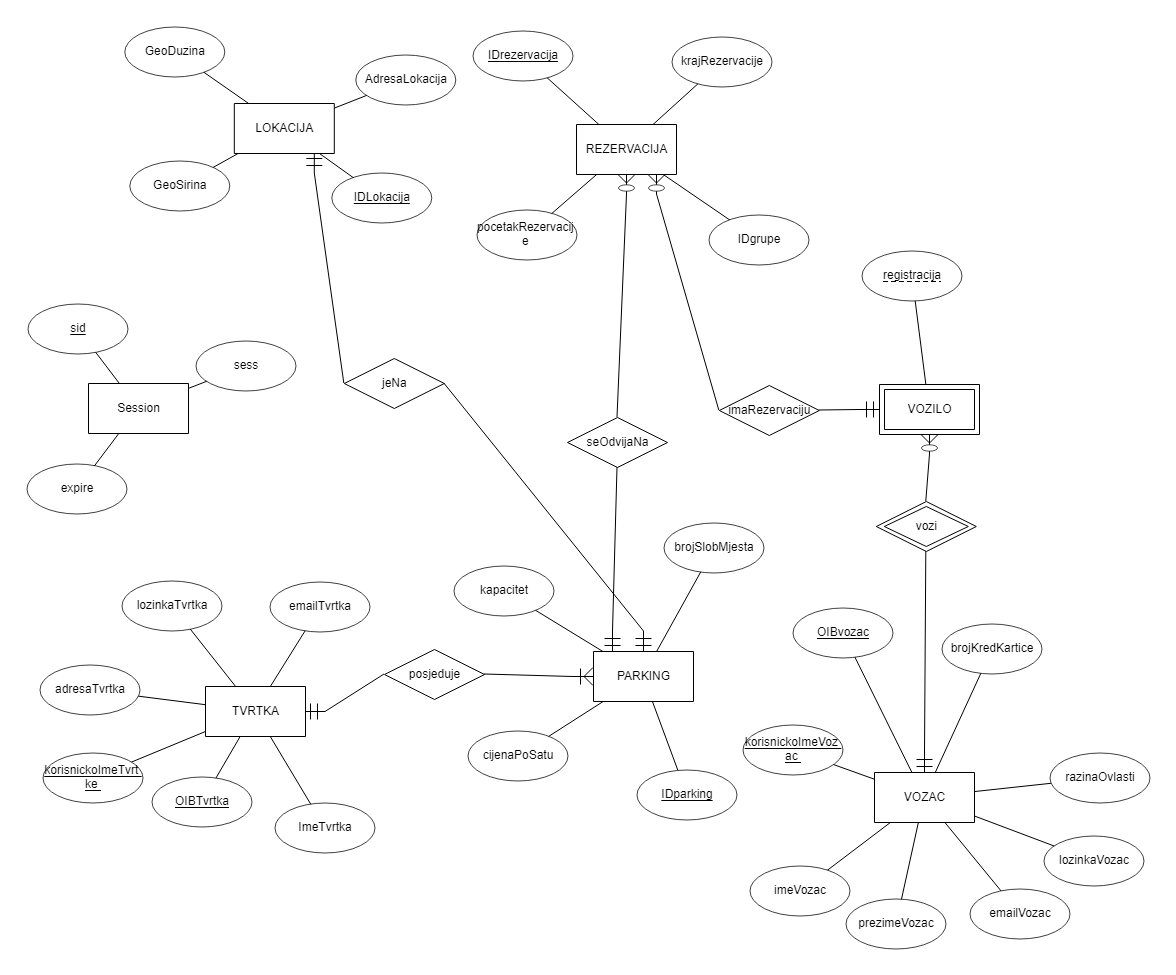
\includegraphics[scale=0.4]{dijagrami/ParkirajMeERModel.png} %veličina slike u odnosu na originalnu datoteku i pozicija slike
					\centering
					\caption{ER model}
					\label{fig:promjene}
				\end{figure}
				

				%unos slike
				\begin{figure}[H]
					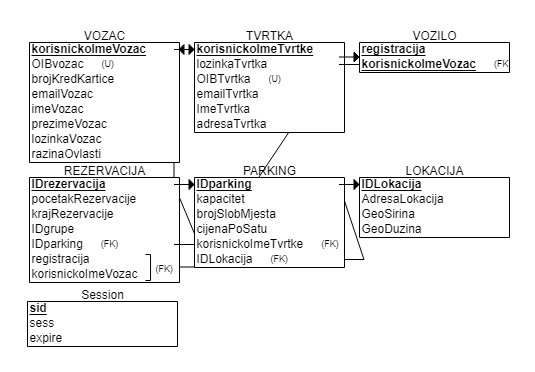
\includegraphics[scale=0.8]{dijagrami/ParkirajMeRelShema.png} %veličina slike u odnosu na originalnu datoteku i pozicija slike
					\centering
					\caption{relacijska shema}
					\label{fig:promjene}
				\end{figure}


			

			\eject
			
			
		\section{Dijagram razreda}
		
			Dijagrami razreda MVC arhitketure sustava prikazani su na slikama 4.4, 4.5 i 4.6.\\
			Razredi na slici 4.3 predstavljaju klase modela, koji su uglavnom direktno povezani s entitetima u bazi podataka. \\
			Razredi na slici 4.4 su pomoćne klase koje pomažu upravljanju podatcima, te najčešće služe za komunikaciju s bazom podataka.\\
 		    Na slici 4.5 se vide razredi koji implementiraju funkcionalnosti \textit{routera}\footnote{https://expressjs.com/en/guide/routing.html}. Oni prikazuju pug\footnote{https://pugjs.org/api/getting-started.html} datoteke koje određuju sadržaj i izgled web stranice.
			\newline
			Razred \textbf{Korisnik} predstavlja bilo kojeg korisnika aplikacije, bio to vozač, tvrtka, administrator ili ne-registrirani korisnik. \textbf{Vozač} predstavlja korisnika aplikacije koji želi rezervirati parirališno mjesto, a \textbf{Tvrtka} korisnika koji želi iznajmljivati svoju parkirališnu površinu. \textbf{Administrator} je korisnik s najvećim ovlastima na aplikaciji. 
			Klasa \textbf{Rezervacija} u sebi pohranjuje informacije o registracijama, kojih postoji 3 različite vrste (jednokratne, ponavljajuće i trajne) koje se označuju atributom \textbf{idgrupe} koja označava pripadajuću vrstu rezervacije:
			\begin{itemize}
				\item jednokratna 	= 0
				\item ponavljajuća 	= 1
				\item trajna 		= 2
			\end{itemize}
			
			%unos slike
			\begin{figure}[H]
				\includegraphics[scale=0.4]{dijagrami/modeli.png} %veličina slike u odnosu na originalnu datoteku i pozicija slike
				\centering
				\caption{Dijagram razreda za modele}
				\label{fig:promjene}
			\end{figure}
		
		
			Pomoćne klase su klase koje u sebi sadrže pomoćne funkcije koje potpomažu ostvarivati funkcionalnosti drugih klasa, te većina služi za direktno slanje upita bazi podataka. Klasa \textbf{datePicker} služi za prikaz izbornika datuma, dok \textbf{displayLocations} služi za prikaz karte preko \textit{Google Maps APIa}, te prikaz lokacija na karti.
			
			%unos slike
			\begin{figure}[H]
				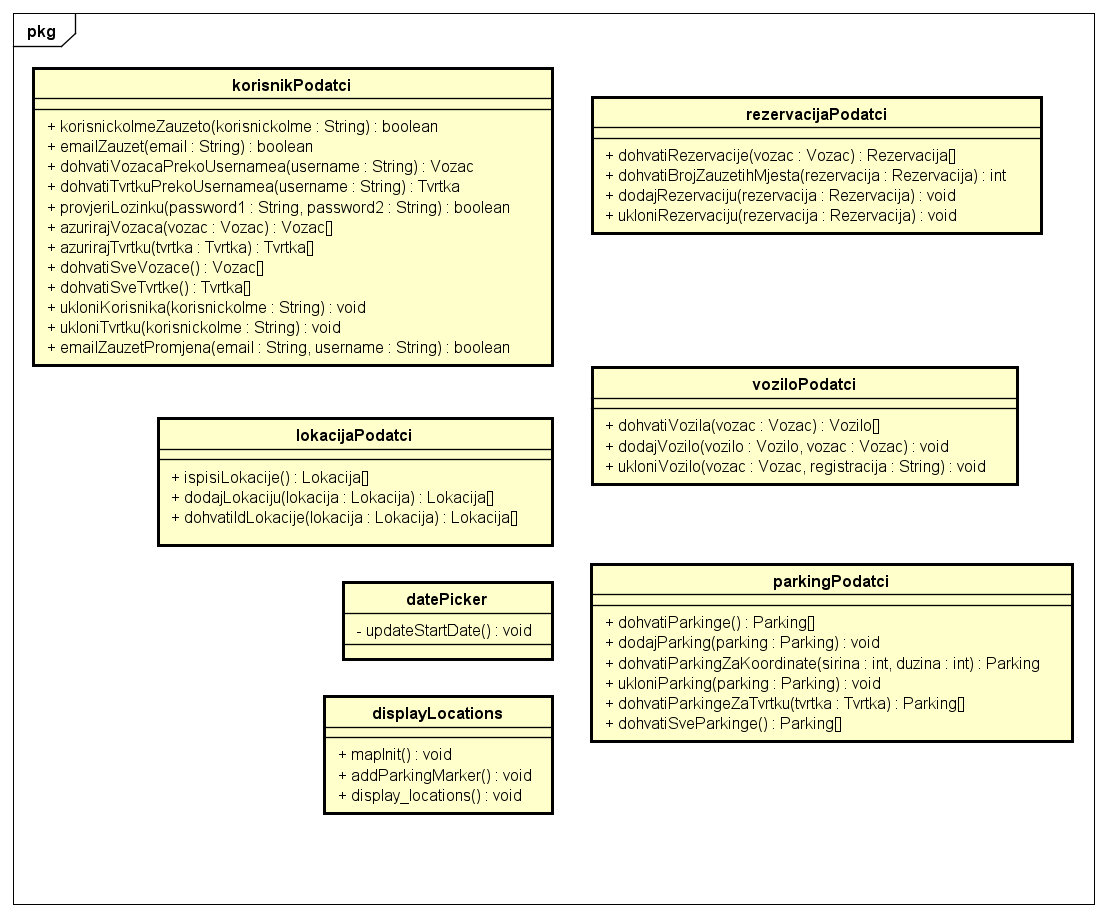
\includegraphics[scale=0.55]{dijagrami/pomocne_funkcije.png} %veličina slike u odnosu na originalnu datoteku i pozicija slike
				\centering
				\caption{Dijagram razreda za pomoćne razrede}
				\label{fig:promjene}
			\end{figure}
		
			\textit{Routeri} su klase koji služe za povezivanje sa \textit{frontendom}, odnosno ostvaruju prikazivanje pug datoteka. Postoje routeri za \textbf{home-page}, stranicu za vozače (\textbf{user.routes}), stranicu za tvrtke (\textbf{company.routes}) te administratora (\textbf{admin.routes}).
			
			\textbf{Napomena:} sve funkcije kao parametre primaju \textit{request} i \textit{response} objekt, te referencu \textit{next} na idući \textit{middleware}\footnote{\textit{middleware} funckije su one funkcije koje imaju pristup \textit{req i res} objektima i idućoj \textit{middleware} funkciji}, no parametri nisu prikazani na dijagramu radi preglednosti.
			
			%unos slike
			\begin{figure}[H]
				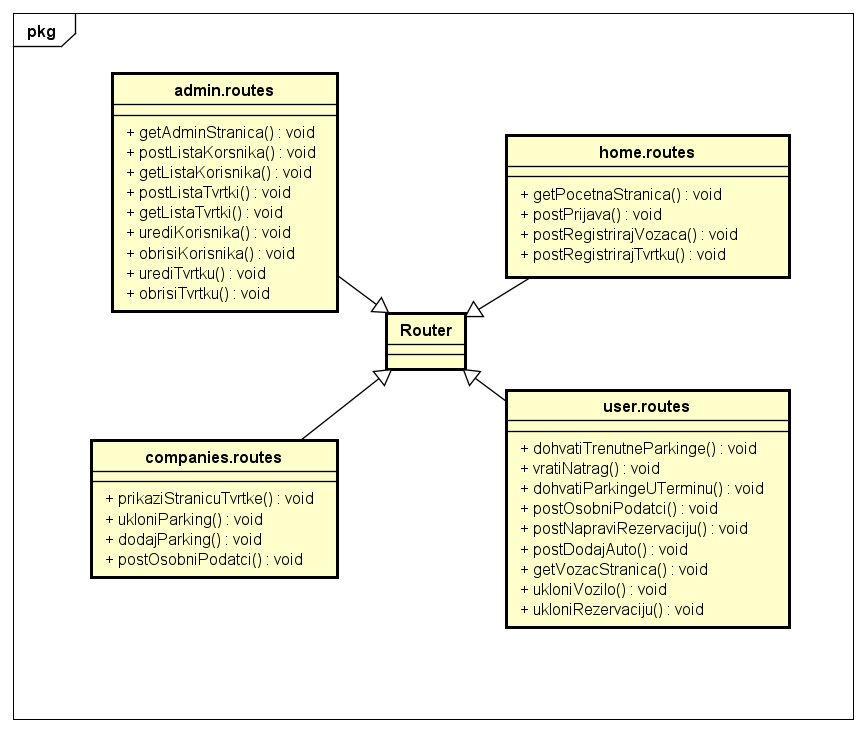
\includegraphics[scale=0.55]{dijagrami/ruteri.png} %veličina slike u odnosu na originalnu datoteku i pozicija slike
				\centering
				\caption{Dijagram razreda za routere}
				\label{fig:promjene}
			\end{figure}
												
			\eject
		
		\section{Dijagram stanja}
			
			Ovaj dijagram stanja prikazuje funkcionalost razreda \textbf{Vozač}. Na web-stranici za vozače (ranije spomenut \textbf{user.routes}) prikazuje se karta pomoću integracije sa \textit{Google Maps APIem}, te više opcija za izabrati koje su naznačene u pravokutnicima. Klik na svaku od njih je otvara, odnosno zatvara te se onda nakon otvaranja prikazuju detalji te opcije. Najkompleksnija opcija je ona za pravljenje rezervacije parking mjesta, jer se u sklopu nje komunicira i sa bazom podataka radi provjere detalja rezervacije i sa poslužiteljem banke gdje se izvršava proces naplate. Greška u bilo kojem dijelu dovršavanja rezervacije otkazuje proces zapisivanja iste u bazu podtaka i njenu naplatu, te usmjerava korisnika nazad na glavnu stranicu gdje može pokušati opet uspješno napraviti rezervaciju.
			
			%unos slike
					\begin{figure}[H]
						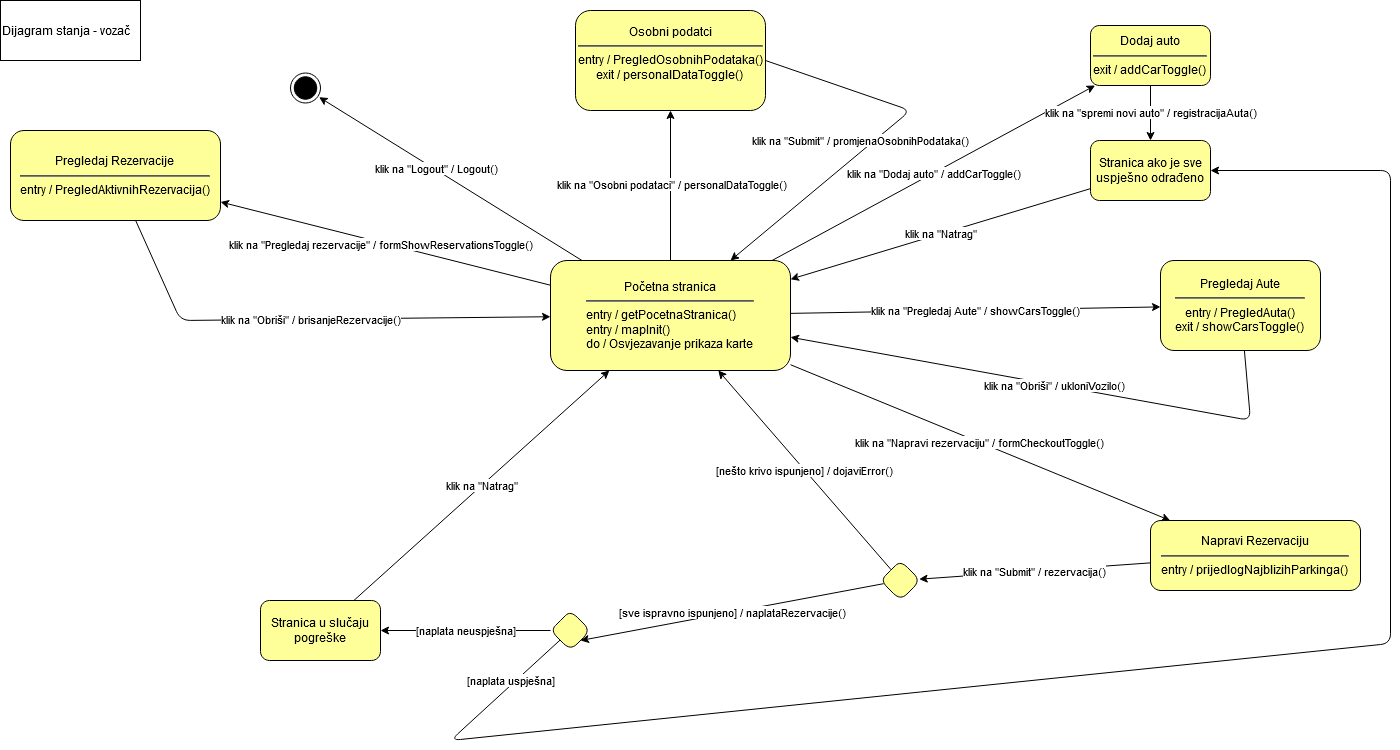
\includegraphics[scale=0.35]{dijagrami/dijagram stanja.png} %veličina slike u odnosu na originalnu datoteku i pozicija slike
						\centering
						\caption{Dijagrama stanja - razred vozač}
						\label{fig:promjene}
					\end{figure}
			
			\eject 
		
		\section{Dijagram aktivnosti}
			 
			 Dio sustava prikazan ovim dijagramom aktivnosti je postupak rezervacije parkinga. Aktivnost započinje (uspješnom) prijavom u sustav. Nakon toga odabire se opcija pravljenja rezervacije gdje se odabire parking i popunjavaju traženi podatci. Važno je napomenuti da se automatski odabire najbliža parking lokacija, koja se onda može ručno izmjeniti po želji korisnika. Nakon ispunjavanja detalja rezervacija se može dovršiti i poslati na naplatu, te ako je sve u redu ona se pamti u bazi podataka i korisnika se obavještava o uspješnoj rezervaciji. Podaci za naplatu se šalju banci na provjeru i izvršavanje naloga pa je neophodno ostvariti sigurnu komunikaciju s tim poslužiteljem radi sigurnosti korisničkih podataka.
			
%unos slike
					\begin{figure}[H]
						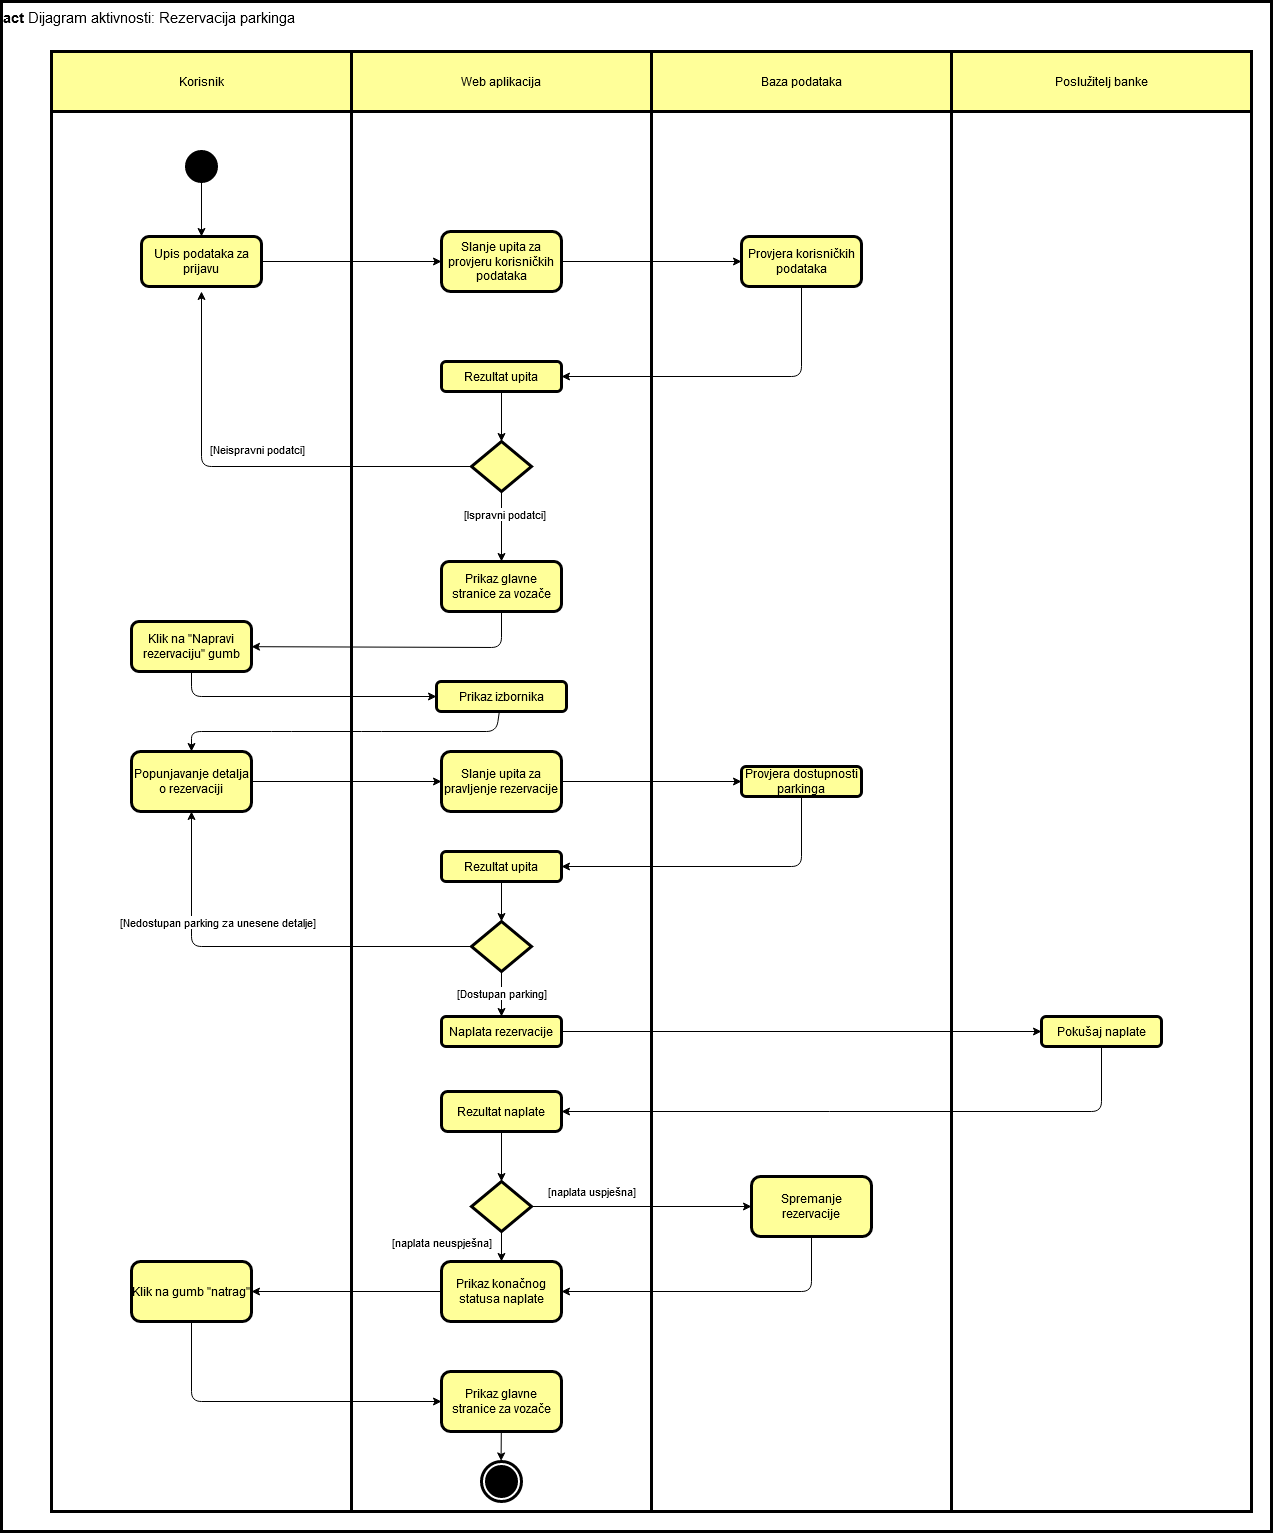
\includegraphics[scale=0.35]{dijagrami/dijagram aktivnosti.png} %veličina slike u odnosu na originalnu datoteku i pozicija slike
						\centering
						\caption{Dijagrama aktivnosti - rezervacija parkinga}
						\label{fig:promjene}
					\end{figure}			
			
			\eject
		\section{Dijagram komponenti}
		
			Na slici je prikazan dijagram komponenti aplikacije. Dijagram prikazuje organizaciju i međuodnos implementacijskih komponenata napravljenih u okviru MVC arhitekture te njihov odnos s okolinom, tj. vanjskim komponentama aplikacije: bazom podataka, \textit{Google Mapsom} i web preglednikom. Web  preglednik komunicira s \textit{routerima} preko REST API  sučelja. Veza između SQL baze podataka i web aplikacije, odnosno njene komponente \textit{podatci} koja dohvađa i obrađuje podatke iz baze podataka, ostvarena je pomoću SQL API sučelja dok je veza s vanjskim servisom \textit{Google Maps} ostavren pomoću GOOGLE MAPS API sučelja.		 
			 
			%unos slike
			 \begin{figure}[H]
				 	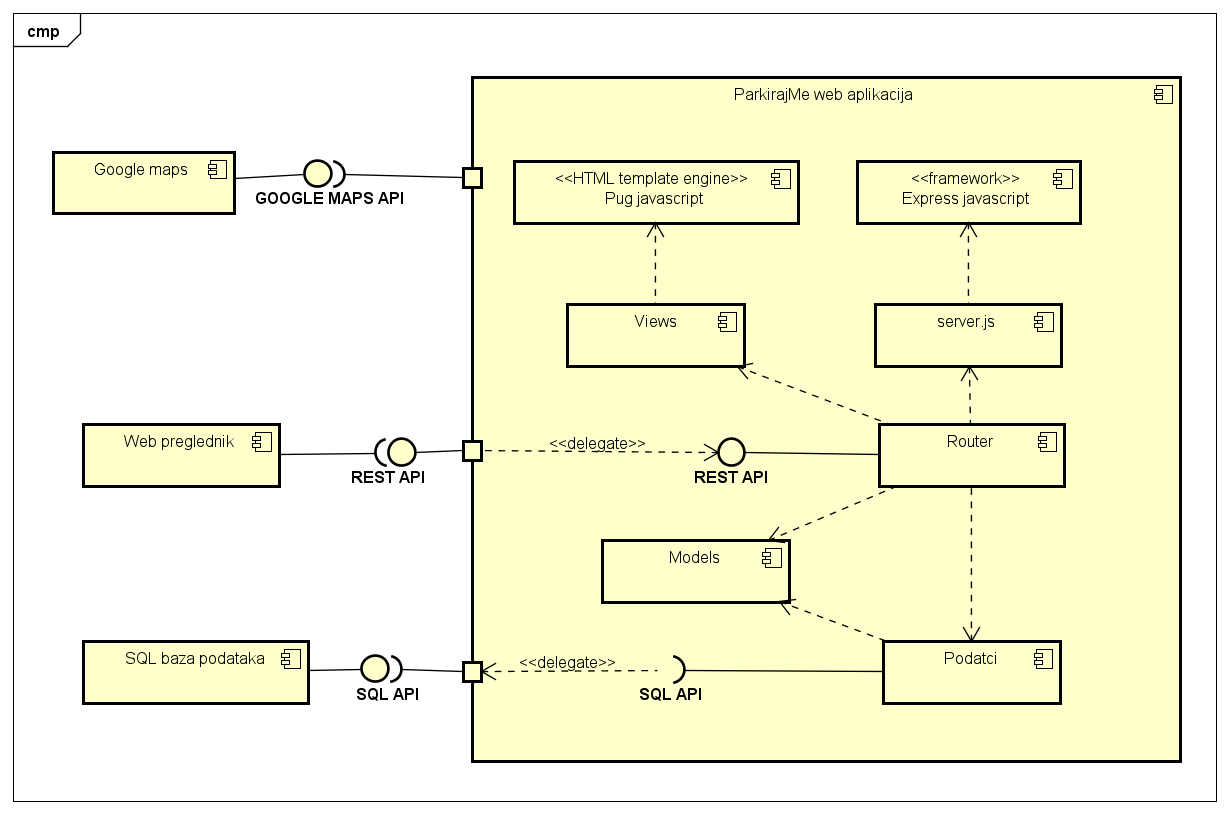
\includegraphics[scale=0.55]{dijagrami/Component Diagram0.png} %veličina slike u odnosu na originalnu datoteku i pozicija slike
				 	\centering
				 	\caption{Dijagram komponenti}
				 	\label{fig:dijagram komponenti}
			 \end{figure}
			 
			 
	\chapter{Implementacija i korisničko sučelje}
		
		
		\section{Korištene tehnologije i alati}
			
			Komunikacija u timu realizirana je korištenjem aplikacija MS Teams\footnote{https://www.microsoft.com/en-us/microsoft-365/microsoft-teams/group-chat-software}, WhatsApp\footnote{https://www.whatsapp.com/?lang=en} i Discord\footnote{https://discord.com/}. Za izradu UML dijagrama korišteni su alati Astah Professional\footnote{astah.net/products/astah-professional/} i Draw.io\footnote{https://app.diagrams.net/}. Kao sustav za upravljanje izvornim kodom korišten je Git\footnote{https://git-scm.com/}, a udaljenom repozitoriju projekta se može pristupiti na web platformi GitLab\footnote{https://gitlab.com/}.
			
			Kao razvojno okruženje korišten je Microsoft Visual Studio Code\footnote{https://code.visualstudio.com/}, te Eclipse\footnote{https://www.eclipse.org/} i IntelliJ\footnote{https://www.jetbrains.com/idea/} za dijelove koda pisane u Javi. Visual Studio Code je besplatan editor izvornog koda razvijen od tvrtke Microsoft za Windows, Linux i macOS. Njegove značajke uključuju podršku za debuggiranje, isticanje sintakse, inteligentno završavanje napisanog koda, refakotoriranje koda i ugrađen Git. IntelliJ i Eclipse su IDEvi razvijeni za programski jezik Java.
			
			Aplikacija je napisana koristeći Express\footnote{https://expressjs.com/} radni okvir i jezik Javascript za izradu backenda te Node.js\footnote{https://nodejs.org/en/} i pug\footnote{https://pugjs.org/api/getting-started.html} za izdradu frontenda. Node.js je kao asikroni i događajima-pokrenut JavaScript runtime dizajniran za izradu skalabilnih web aplikacija. Pug je HTML-ov predprocesor.
			
			Za prikaz karte i lokacije parkinga korišten je Google Maps api\footnote{https://developers.google.com/maps/documentation/javascript/overview}. Za potrebe baze podataka korišten je PostgreSQL\footnote{https://www.postgresql.org/}. Sama aplikacija i baza podataka je objavljena na cloud platformi Heroku\footnote{https://www.heroku.com/}.
			
			Za potrebe sistemskog testiranja aplikacije korišten je Selenium\footnote{https://www.selenium.dev/} i jezik Python (koristeno razvojno okruzenje Pycharm\footnote{https://www.jetbrains.com/pycharm/}). Selenium je prijenosni radni okvir za testiranje web aplikacija. Pruža alat za pravljenje funkcionalnih testova bez potrebe da se uči skriptni jezik za testiranje.\newline
			Za testiranje Node.js funkcija korišten je Mocha\footnote{https://mochajs.org/}. Kao napredni uređivač teksta korišten je Sublime\footnote{https://www.sublimetext.com/}.
			
			
			\eject 
		
	
		\section{Ispitivanje programskog rješenja}
							
			Ispitivanje (testiranje) se provelo u dva oblika. Prvi je kroz sistemske, a drugi kroz \textit{unit} testove. 
			Sistemskim testovima testiran je dio sustava (aplikacije), a \textit{unit} testovima manji segment (funkcija) u kodu.
			
			Sistemskim testovima provjerena je funkcionalnost registracije korisnika, registracija tvrtke, prijava korisnika, prijava tvrtke, dodavanje automobila (korisnička funkcionalnost) te promjena imena (korisnička funkcionalnost).
			
		
			
			
			\subsection{Ispitivanje komponenti}
			
			Testiranje je obavljeno u Node.js-u pomoću Mocha-e.\newline
			
			Testiranjem komponenti željelo se provjeriti ispravnost funkcija napisanih na klijentskoj strani. Ovim testovima provjeravalo se dohvaćanje korisničkih podataka (ime i prezime), dohvaćanje lokacije (preko ID-a i koordinata), dohvaćanje rezervacija i dohvaćanje vozila.\newline
			
			U nastavku je prikazan kod i rezultati testiranja.
	
			%unos slike
			\begin{figure}[H]
				\begin{lstlisting}
					const assert = require('chai').assert;
					const KorisnikPodatci = require('../tools/KorisnikPodatci');
					
					describe('KorisnikPodatci', async function(){
						it('Trebao bi vratiti test', async function(){
							const vozac = await KorisnikPodatci.dohvatiVozacaPrekoUsernamea('testuser');
							assert.equal(vozac.imeVozac, 'test');
						});
						
						it('Trebao bi vratiti test', async function(){
							const vozac = await KorisnikPodatci.dohvatiVozacaPrekoUsernamea('testuser');
							assert.equal(vozac.prezimeVozac, 'test');
						});
					});
				\end{lstlisting}
				
				\centering
				\caption{Prikaz testa dohvaćanja korisničkih podataka}
				\label{fig:test - user - dohvacanje korisničkih podataka}
			\end{figure}
	

	


			%unos slike
			\begin{figure}[H]
				\begin{lstlisting}
					const assert = require('chai').assert;
					const LokacijaPodatci = require('../tools/LokacijaPodatci');
					const Lokacija = require('../models/Lokacija')
					
					describe('LokacijaPodatci', async function(){
						it('Trebao bi vratiti 36', async function(){
							lokacijaBezId = new Lokacija('trg bana josipa jelacica', 45.813264153294114, 15.977233094526218);
							const lokacija= await LokacijaPodatci.dohvatiIdLokacije(lokacijaBezId);
							assert.equal(lokacija[0].idlokacija, 36);
						});
					});
				\end{lstlisting}
			
				\centering
				\caption{Prikaz testa dohvaćanja lokacije preko id-a}
				\label{fig:test - user - dohvaćanje lokacije preko id-a}
			\end{figure}
				
			%unos slike
			\begin{figure}[H]
				
				\begin{lstlisting}
					const assert = require('chai').assert;
					const ParkingPodatci = require('../tools/ParkingPodatci');
					
					describe('LokacijaPodatci', async function(){
						it('Postoje dva parkinga sa istom lokacijom \
						(moze se dogodit da neka tvrtka slucajno doda),\
						pa se vraca samo jedna', async function(){
							//jelacic koordinate, ima dvije lokacije
							let parking = await ParkingPodatci.dohvatiParkingZaKoordinate(
							45.813264153294114, 15.977233094526218);
							assert.equal(parking.idlokacija, 35);
						});
					});
				\end{lstlisting}
				
				\centering
				\caption{Prikaz testa dohvaćanja lokacije preko koordinata}
				\label{fig:test - user - dohvaćanje lokacije preko koordinata}
			\end{figure}
				
			%unos slike
			\begin{figure}[H]
				
				\begin{lstlisting}
					const assert = require('chai').assert;
					const RezervacijaPodatci = require('../tools/RezervacijaPodatci');
					const KorisnikPodatci = require('../tools/KorisnikPodatci');
					
					
					describe('RezervacijaPodatci', async function(){
						it('Trebao bi vratiti sava, tvrtka, 500, test', async function(){
							vozac = await KorisnikPodatci.dohvatiVozacaPrekoUsernamea('testuser')
							rezervacije = await RezervacijaPodatci.dohvatiRezervacije(vozac);
							assert.equal(rezervacije[0].adresalokacija, 'sava');
							assert.equal(rezervacije[0].korisnickoimetvrtke, 'tvrtka');
							assert.equal(rezervacije[0].kapacitet, 500);
							assert.equal(rezervacije[0].registracija, 'test');
						});
					});
				\end{lstlisting}
			
				\centering
				\caption{Prikaz testa dohvaćanja rezervacija}
				\label{fig:test - user - dohvaćanje rezervacija}
			\end{figure}
				
			%unos slike
			\begin{figure}[H]
				\begin{lstlisting}
					const assert = require('chai').assert;
					const VoziloPodatci = require('../tools/VoziloPodatci');
					const KorisnikPodatci = require('../tools/KorisnikPodatci');
					const Vozilo = require('../models/Vozilo')
					const chai = require('chai')
					const expect = chai.expect
					chai.use(require('chai-as-promised'))
					
					describe('VoziloPodatci', async function(){
						it('Trebao bi vratiti test, auto1, auto2', async function(){
							vozac = await KorisnikPodatci.dohvatiVozacaPrekoUsernamea('testuser')
							const vozila = await VoziloPodatci.dohvatiVozila(vozac);
							assert.equal(vozila[0].registracija, 'test');
							assert.equal(vozila[1].registracija, 'auto1');
							assert.equal(vozila[2].registracija, 'auto2');
						});
						
						it('Trebao bi vratiti 4, 3, noviauto', async function(){
							vozac = await KorisnikPodatci.dohvatiVozacaPrekoUsernamea('testuser')
							vozilo = new Vozilo('noviauto', vozac);
							await VoziloPodatci.dodajVozilo(vozilo, vozac);
							let vozila = await VoziloPodatci.dohvatiVozila(vozac);
							assert.equal(vozila.length, 4);
							await VoziloPodatci.ukloniVozilo(vozac, 'noviauto');
							vozila = await VoziloPodatci.dohvatiVozila(vozac);
							assert.equal(vozila.length, 3);
						});
						
						it('Trebao bi biti error', async function(){
							vozac = await KorisnikPodatci.dohvatiVozacaPrekoUsernamea('testuser')
							vozilo = new Vozilo('   ', vozac);
							await expect(VoziloPodatci.dodajVozilo(vozilo, vozac)).to.be.rejectedWith(Error)
						});
						
					});
				\end{lstlisting}
				
			
				\centering
				\caption{Prikaz testa dohvaćanje vozila}
				\label{fig:test - user - dohvaćanje vozila}
			\end{figure}
				
			%unos slike
			\begin{figure}[H]
				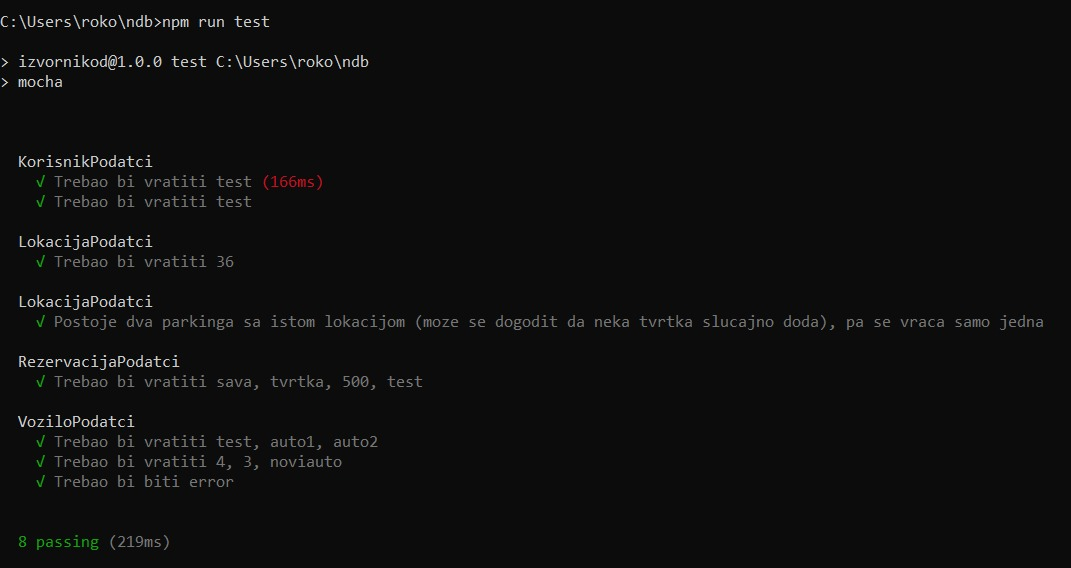
\includegraphics[scale=0.4]{slike/test_unit_testsOK.jpg} %veličina slike u odnosu na originalnu datoteku i pozicija slike
				\centering
				\caption{Prikaz prolaza svih testova}
				\label{fig:test - user - prolaz svih testova}
			\end{figure}
	
			%unos slike
			\begin{figure}[H]
				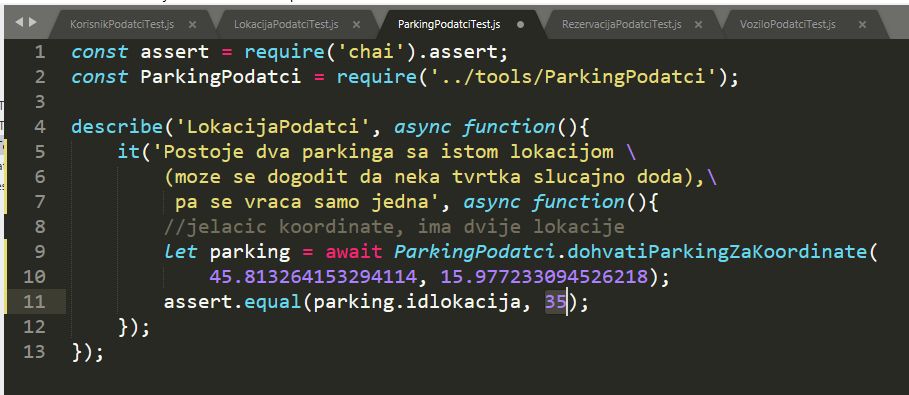
\includegraphics[scale=0.6]{slike/test_unit_kriviTest.png} %veličina slike u odnosu na originalnu datoteku i pozicija slike
				\centering
				\caption{Prikaz testa u kojem se očekuje drugačija vrijednost od dobivene (označena razlika u odnosu na prijašnji test)}
				\label{fig:test - user - test s neocekivanom vrijednosti}
			\end{figure}		
		
		
			%unos slike
			\begin{figure}[H]
				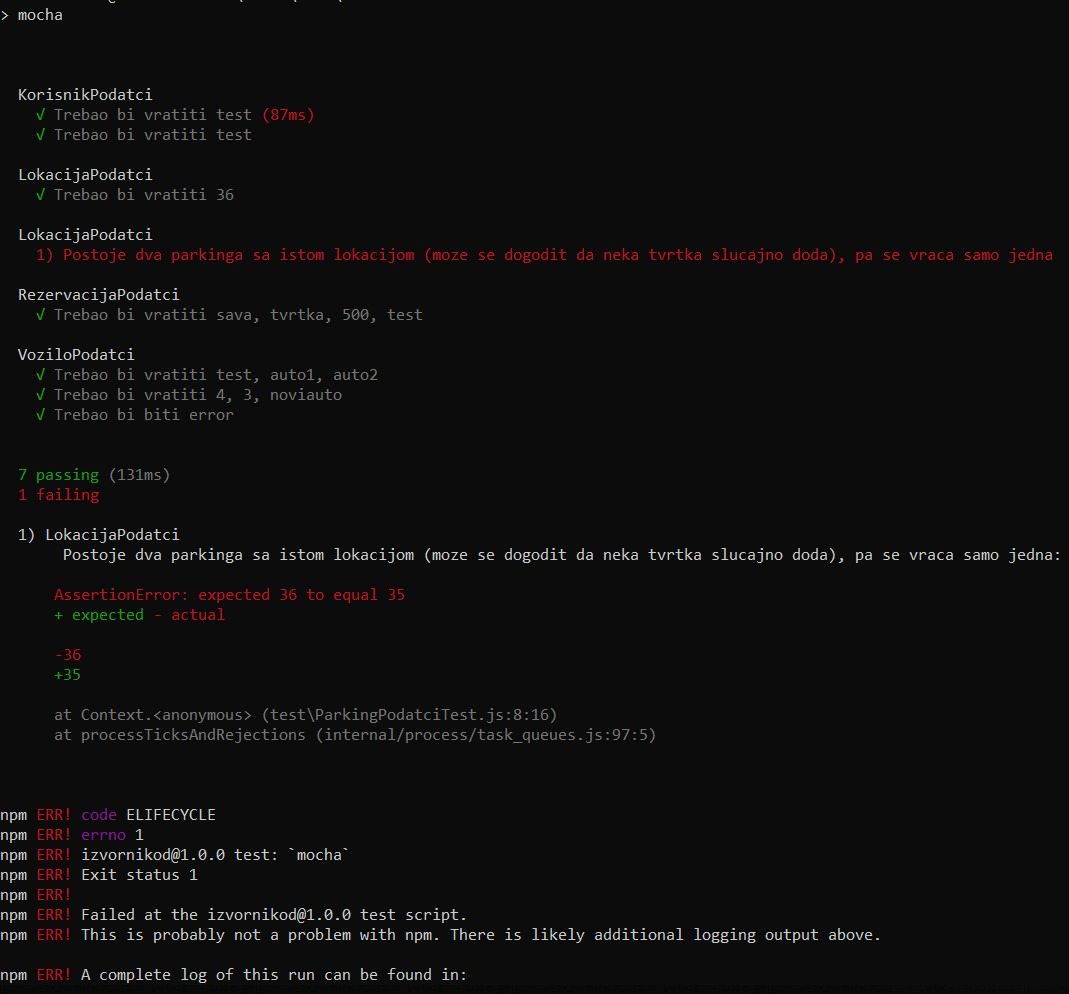
\includegraphics[scale=0.4]{slike/test_unit_testNeOK.jpg} %veličina slike u odnosu na originalnu datoteku i pozicija slike
				\centering
				\caption{Prikaz neprolaženja svih testova}
				\label{fig:test - user - neprolazenje svih testova}
			\end{figure}	
				
			\subsection{Ispitivanje sustava}
							
					Kod za testiranje je pisan u Pythonu, Selenium je korišten za interakciju s elementima u aplikaciji.
			
			Kao pripremu za testiranje registracija napravljene su baze podataka koje sadrže nasumično generirane parametre (ime, prezime, broj kartice i slično). Prilikom registracije dohvaća se jedan set podataka koji se koriste za registraciju te se nakon toga bilježi kako su ti podatci iskorišteni, pri idućoj registraciji dohvaća se novi set podataka. Proces je iterativan. 
			Razlog ovakvog pristupa naspram ustaljenog (procedure koja prije pokretanja testa registracije briše testnog korisnika ili tvrtku kako bi se mogao ponovno koristiti taj isti korisnik ili tvrtka za registraciju) je što se ovako ostvaruje dualna funkcija; \underline{testiranje} i \underline{pisanje} podataka u bazu. Drugo ima za posljedicu lakše ručno testiranje svih funkcionalnosti vezanih uz korisnike i tvrtke pošto su već upisani u bazi te se ne treba stvarati ispitni skup korisnika i tvrki (na primjer: kako bi se testirale administratorske ovlasti nad njima)
			
			Druga priprema koja je napravljena na \textit{home} stranici je pridruživanje svakom relevantnom elementu za testiranje \textit{id}. Svaki \textit{id} je broj, te su vrijednosti posložene tako da se pri testiranju može iterirati po određenom spektru tih brojeva i jednostavno dohvaćati elemente, pritiskati na njih i upisivati u njih željene znakove. 
					
			
			%unos slike
			\begin{figure}[H]
				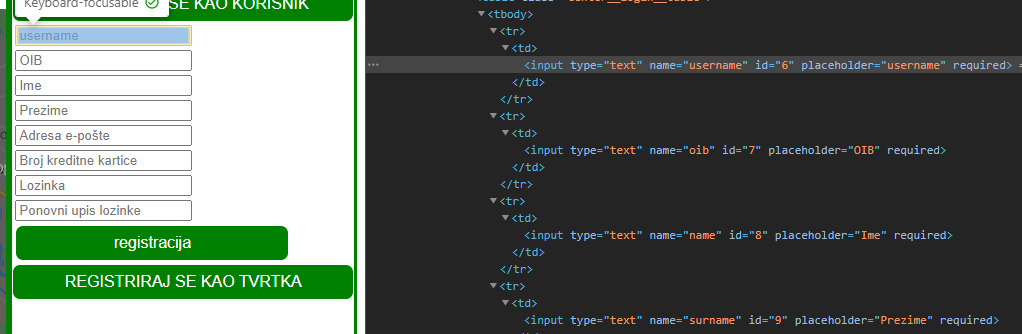
\includegraphics[scale=0.6]{slike/html_id.png} %veličina slike u odnosu na originalnu datoteku i pozicija slike
				\centering
				\caption{Prikaz enumeracije \textit{id}-eva}
				\label{fig:promjene}
			\end{figure}
		
			U nastavku je prikaz koda i rezultata testiranja.
			Većina testova koristi \textit{driver} koji obavlja test s predanim parametrima koje mu određeni test predaje.
			Svi testovi se nalaze u klasi \textit{TestApp}.
			
			%unos slike
			\begin{figure}[H]
				\begin{lstlisting}
				# ... importi
				
				class TestApp(unittest.TestCase):
				
					PAGE_URL = "http://127.0.0.1:3000/"
					SHOW_LOG = False
					USER_USERNAME = "marin"
					USER_PASSWORD = "123123"
					
					IS_ALL_OK = True
					
					driver = webdriver.Chrome(ChromeDriverManager().install())
					
				# ... nastavak koda
				\end{lstlisting}
		
				\centering
				\caption{Prikaz varijabli i konstanti}
				\label{fig:test - sistemski- varijable i konstante}
			\end{figure}
		
					
			%unos slike
			\begin{figure}[H]
				
				\begin{lstlisting}
					# ... unutar TestApp
					
					def login_driver(self, username, password, invert_score=False):
						driver = self.driver
						
						try:
							driver.get(self.PAGE_URL)
							time.sleep(4)
							
							i_0 = 2
							credentials = [username, password]
							
							for i_1 in credentials:
								user = driver.find_element_by_id(i_0)
								user.click()
								user.send_keys(i_1)
								i_0 += 1
							
							user = driver.find_element_by_id(i_0)
							user.click()
							
							time.sleep(4)
							try:
								tester = driver.find_element_by_id("name_ph")
							except:
								raise self.FailTest("login nije uspjesno napravljen")
								
							self.assertTrue(not invert_score)
							
						except self.FailTest as e:
							self.IS_ALL_OK = False
							print(e)
							
							self.assertTrue(invert_score)
							
						except:
							self.IS_ALL_OK = False
							import sys
							print(sys.exc_info()[0])
							self.assertTrue(False)
				\end{lstlisting}
				
				\centering
				\caption{Prikaz login drivera}
				\label{fig:test - sistemski - login driver}
			\end{figure}

			%unos slike
			\begin{figure}[H]
				\begin{lstlisting}
					# ... unutar TestApp
				    def test_login_user_false(self):
						username = "marin"
						password = "123d123"
						
						self.login_driver(username, password, True)	
			
				\end{lstlisting}
				
			
				\centering
				\caption{Prikaz testa koji ne uspjeva se prijaviti u aplikaciji}
				\label{fig:test - sistemski - neuspjela prijava korisnika}
			\end{figure}			
			\eject 
		
			%unos slike
			\begin{figure}[H]
								\begin{lstlisting}
					# ... unutar TestApp
					def test_user_change_name(self):
					
						try:
							self.login_driver(self.USER_USERNAME, self.USER_PASSWORD)
							
							if self.IS_ALL_OK:
							
								
								time.sleep(4)
								
								self.driver.find_element_by_id(0).click()
								time.sleep(1)
								
								self.driver.find_element_by_id("firstname").click()
								self.driver.find_element_by_id("firstname").clear()
								self.driver.find_element_by_id("firstname").\
									send_keys(get_user_first_name())
								
								self.driver.find_element_by_id(4).click()
								
								self.assertTrue(True)
							
							else:
								raise self.FailTest("login nije uspjesno napravljen")
						
						
						except:
							self.assertTrue(False)
					
				\end{lstlisting}
				
			
				\centering
				\caption{Prikaz testa promjena imena korisnika}
				\label{fig:test - sistemski - promjena imena korisnika}
			\end{figure}		
		

			%unos slike
			\begin{figure}[H]
								\begin{lstlisting}
					# ... unutar TestApp
					
					def test_user_add_car(self):
					
					try:
						self.login_driver(self.USER_USERNAME, self.USER_PASSWORD)
						if self.IS_ALL_OK:
						
							time.sleep(4)
							
							self.driver.find_element_by_id("addCar").click()
							time.sleep(1)
							
							self.driver.find_element_by_id("addCarInputField").click()
							self.driver.find_element_by_id("addCarInputField").\
								send_keys(get_user_licence_plate("zg_plate"))
							
							self.driver.find_element_by_id("addCarButton").click()
							
							self.assertTrue(True)
						
						else:
							raise self.FailTest("login nije uspjesno napravljen")
					
					except:
						self.assertTrue(False)
				\end{lstlisting}
			
				\centering
				\caption{Prikaz testa dodavanja automobila}
				\label{fig:test - sistemski - dodavanje automobila}
			\end{figure}			

			
			%unos slike
			\begin{figure}[H]
								\begin{lstlisting}
					# ... unutar TestApp
	   				def test_login_user(self):
					
						username = "marin"
						password = "123123"
						
						self.login_driver(username, password)
						
  					def test_login_company(self):
						
						username = "marin doo"
						password = "123123d"
						
						self.login_driver(username, password)
						
				\end{lstlisting}
			
				\centering
				\caption{Prikaz testova za prijavu (korisnika i tvrtke)}
				\label{fig:test - sistemski - prijava}
			\end{figure}		

			
			%unos slike
			\begin{figure}[H]
								\begin{lstlisting}
					# ... unutar TestApp
					def signup_user_driver(self, plate_tag):
						driver = self.driver
						credentials = [
							get_user_username(), get_user_oib(), 
							get_user_first_name(), get_user_last_name(), 
							get_user_email(), get_user_licence_plate(plate_tag),
							get_user_card(), get_user_password()
						]
						if self.SHOW_LOG:
							print(credentials)
						try:
							driver.get(self.PAGE_URL)
							time.sleep(4)							
							i_0 = 5							
							user = driver.find_element_by_id(str(i_0))
							user.click()
							i_0 += 1							
							password = credentials[-1]
							for i_1 in credentials:
								user = driver.find_element_by_id(str(i_0))
								user.click()
								i_0 += 1
								user.send_keys(i_1)
								if self.SHOW_LOG:
									print(i_1)							
							user = driver.find_element_by_id(str(i_0))
							user.click()
							i_0 += 1
							user.send_keys(password)
							user = driver.find_element_by_id(str(i_0))
							user.click()							
							time.sleep(4)							
							try:
								tester = driver.find_element_by_id("name_ph")
							except:
								raise self.FailTest("login nije uspjesno napravljen")
							self.assertTrue(True)							
						except self.FailTest as e:
							print(e)							
							self.assertTrue(False)
						except:
							import sys
							print(sys.exc_info()[0])
							self.assertTrue(False)
				\end{lstlisting}
	
				\centering
				\caption{Prikaz drivera za registraciju korisnika}
				\label{fig:test - sistemski - driver za registraciju korisnika}
			\end{figure}		
			
						
			%unos slike
			\begin{figure}[H]
								\begin{lstlisting}
					# ... unutar TestApp
	    			# zg plate
					def test_signup_user_1(self):
					
						self.signup_user_driver("zg_plate")
					
					# cro plates
					def test_signup_user_2(self):
					
						self.signup_user_driver("cro_plates")
					
					# international_plate
					def test_signup_user_3(self):
					
						self.signup_user_driver("international_plate")
					
				\end{lstlisting}
			
				\centering
				\caption{Prikaz registracije korisnika s različitim registracijama automobila}
				\label{fig:test - sistemski - registracija korisnika}
			\end{figure}		
			
						
			%unos slike
			\begin{figure}[H]
								\begin{lstlisting}
					# ... unutar TestApp
	    			def test_signup_company(self):
						driver = self.driver
						
						credentials = [
							get_company_oib(), get_company_name(), 
							get_company_address(), get_company_email(), 
							get_password()
						]
						
						try:
							driver.get(self.PAGE_URL)
							time.sleep(4)							
							i_0 = 16							
							# button: register as company
							user = driver.find_element_by_id(str(i_0))
							user.click()
							i_0 += 1							
							password = credentials[-1]
							if self.SHOW_LOG:
								print("password " + str(password))							
							for i_1 in credentials:
								user = driver.find_element_by_id(str(i_0))
								user.click()
								i_0 += 1
								user.send_keys(i_1)
								if self.SHOW_LOG:
									print(i_1)							
							user = driver.find_element_by_id(str(i_0))
							user.click()
							i_0 += 1
							user.send_keys(password)							
							user = driver.find_element_by_id(str(i_0))
							user.click()							
							time.sleep(4)							
							try:
								tester = driver.find_element_by_id("name_ph")
							except:
								raise self.FailTest("login nije uspjesno napravljen")
							self.assertTrue(True)
						except self.FailTest as e:
							print(e)
							self.assertTrue(False)
						except:
							import sys
							print(sys.exc_info()[0])
							self.assertTrue(False)	
				\end{lstlisting}
	
				\centering
				\caption{Prikaz testa za registraciju tvrtke}
				\label{fig:test - sistemski - registracija tvrtke }
			\end{figure}		
			
			%unos slike
			\begin{figure}[H]
				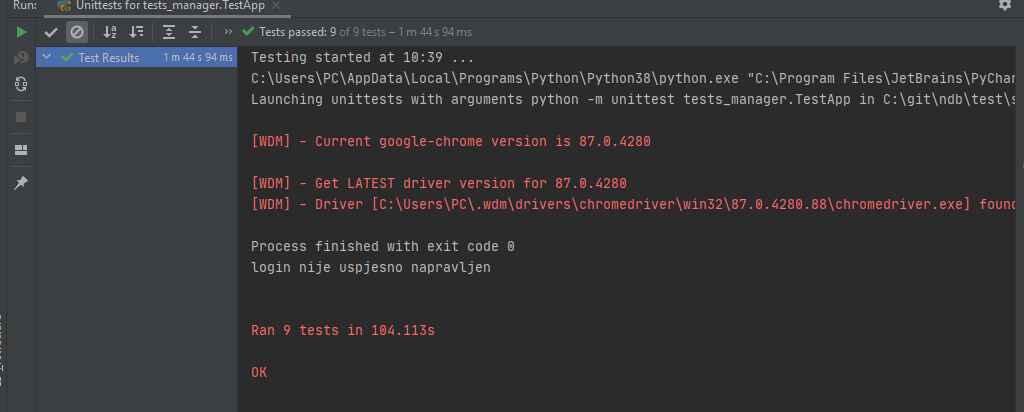
\includegraphics[scale=0.6]{slike/test_sistem_rezultat.png} %veličina slike u odnosu na originalnu datoteku i pozicija slike
				\centering
				\caption{Prikaz rezultata nakon provedenog ispitivanja}
				\label{fig:test - sistemski - rezultat}
			\end{figure}					
	
			%unos slike
			\begin{figure}[H]
				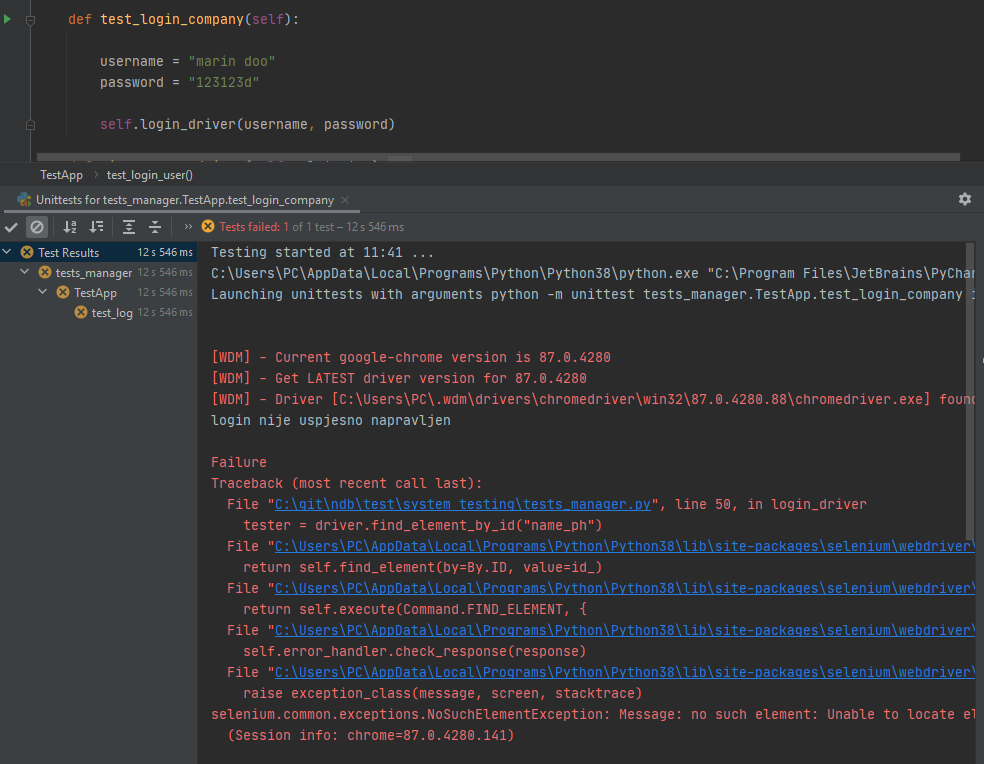
\includegraphics[scale=0.6]{slike/test_sistem_failedTest.png} %veličina slike u odnosu na originalnu datoteku i pozicija slike
				\centering
				\caption{Prikaz primjera rezultata u slučaju da očekujemo rezultat drugačiji od dobivenog (provedeni test je prikazani)}
				\label{fig:test - sistemski - neuspješno provedeni test}
			\end{figure}					
			
			\eject 
		
		
		\section{Dijagram razmještaja}
			 
			 Dijagram razmještaja je strukturni UML dijagram koji opisuje topologiju sustava i prikazuje odnos između sklopovskih i programskih dijelova. Poslužiteljsku stranu predstavlja \textit{cloud} platforma Heroku. Na Heroku se nalaze web poslužitelj i poslužitelj baze podataka, a pristupa kartama omogućen je preko \textit{Google API} servisa. Na klijentskoj strani koristi se web preglednik kojim se pristupa web aplikaciji. Komunikacija između korisnika i oblaka odvija se putem HTTPS veze.
			
			\begin{figure}[H]
				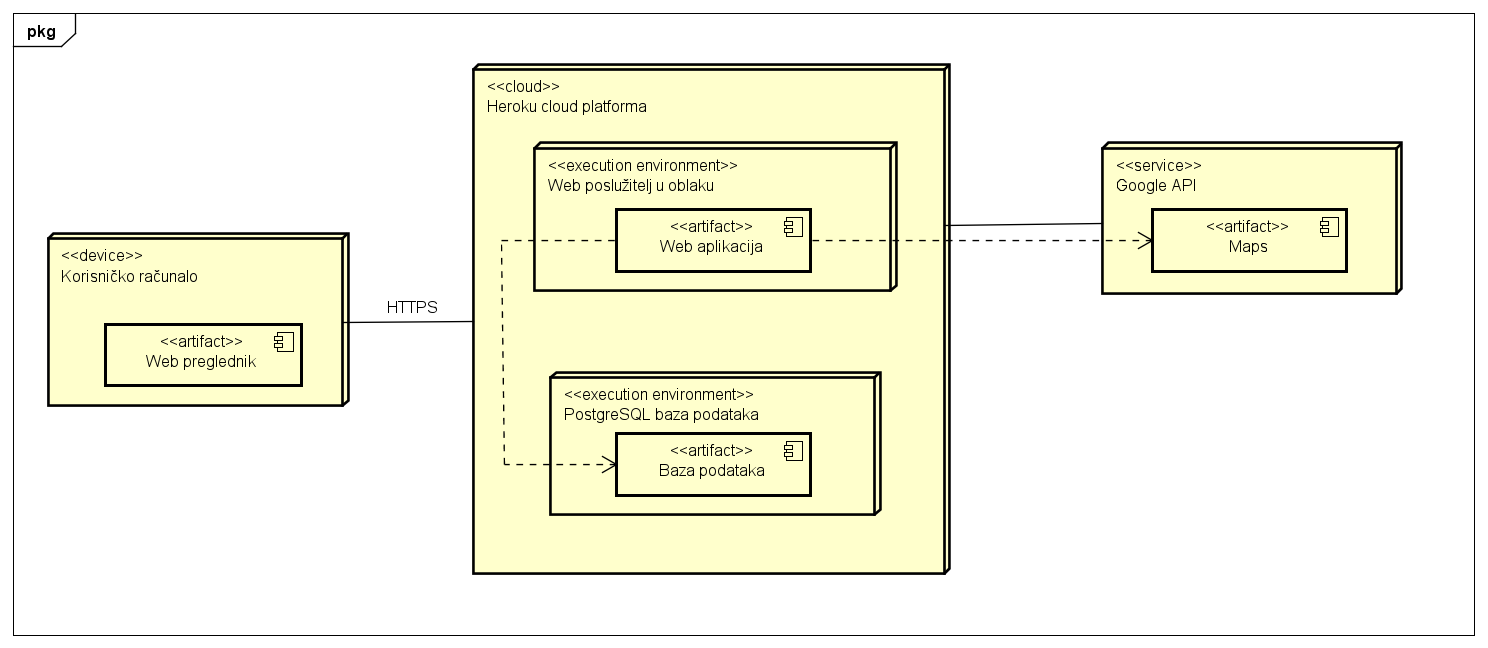
\includegraphics[scale=0.45]{dijagrami/dijagram_razmjestaja.png} %veličina slike u odnosu na originalnu datoteku i pozicija slike
				\centering
				\caption{Dijagram razmještaja}
				\label{fig:promjene}
			\end{figure}
			
			\eject 
		
		\section{Upute za puštanje u pogon}
		
		
			Pokretanje Stranice preko Heroku-a:
			\begin{itemize}
				\item 	\textit{Prvo se treba ulogirati na Heroku}
				\item 	\textit{Nakon logina treba se povezati postojeći git repozitorij sa Heroku-om pozivanjem
					“heroku git:remote -a imestranice”}
				\item 	\textit{Nakon povezivanja repozitorij se može pushati sa “git push heroku master” u slučaju da se pusha sa Master brancha ili “git push heroku imebrancha:master”}		
				
				\item 	\textit{Nakon što se repozitorij pusha na Heroku, potrebno je napraviti bazu podataka.}	
				
				\item 	\textit{Na Resources stranici Heroku-a kao add-on se doda Heroku Postgres te se iz dane baze trebaju uzeti podatci za spajanje}
				
				\item 	\textit{Nakon toga se u konzoli pozove “heroku run bash” kojim se otvori bash te se u bashu pokrene seed.js kako bi se napravila baza podataka}
	
				\item 	\textit{Kada je to napravljeno, web stranica se može pokrenuti}
			\end{itemize}
		
		
			

		
					%unos slike
		\begin{figure}[H]
			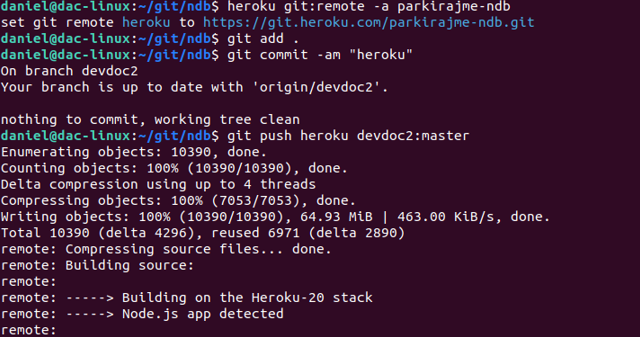
\includegraphics[scale=0.8]{slike/heroku_s1.png} %veličina slike u odnosu na originalnu datoteku i pozicija slike
			\centering
			\caption{Upravljanje Heroku-om}
			\label{fig:Upravljanje Heroku-om 1}
		\end{figure}
	
				%unos slike
	\begin{figure}[H]
		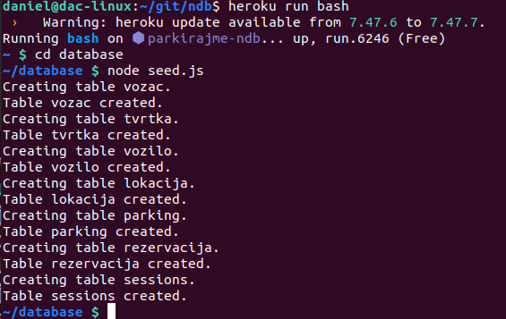
\includegraphics[scale=0.8]{slike/heroku_s2.png} %veličina slike u odnosu na originalnu datoteku i pozicija slike
		\centering
		\caption{Kreiranje baze podataka}
		\label{fig:Upravljanje Heroku-om 2}
	\end{figure}
			
			\eject 
	\chapter{Zaključak i budući rad}
			
		Izrada aplikacije je započeta analiziranjem zadanih uvjeta te pretakanjem korisničkih zahtjeva u formalne zapise uvjeta. Prilikom popisivanja zahtjeva dodani su zahtjevi koje smo smatrali da bi bili od koristi korisnicima. Kasnije se pokazalo da to nije bio dobar potez. \newline
		Nakon formaliziranja zahtjeva korisnika izrađen je kostur aplikacije te su isprobane jednostavne funkcije.\newline
		Ovime je završila prva faza projekta. Dobar potez je bio što smo simultano radili na aplikaciji i usklađivali zahtjeve u dokumentaciji. Loš potez je bio što smo pri izradi kostura krenuli s izradom CSS-a za stranicu što sada smatramo da je trebalo napraviti na kraju. Problem nam je predstavljalo nepoznavanje tehnologije git zbog čega smo puno vremena gubili na raznim konfliktima. Prvi put smo se susreli s Google maps API-jem te je bilo potrebno neko vrijeme da se naviknemo na rad s njim; sada se osjećamo ugodno raditi s njim.
		
		U drugoj fazi projekta smo dovršili aplikaciju i kod. Puno smo se sigurnije osjećali eksperimentirati s tehnologijama pošto smo stekli iskustvo. Ovo je vrlo vjerojatno iz razloga što nismo odlagali izradu za pred rok puštanja u pogon već smo radili kontinuirani pa smo imali vremena i popraviti ako nešto krivo napravimo.\newline
		
		Kako je kod aplikacije postao opsežniji tako smo počeli imati sve više konflikata koje smo rješavali tako što smo prestali u isto vrijeme raditi na istim datotekama. Razlog velikog broja konflikata i gubljenja vremena je što su se često implementirale funkcionalnosti koje su loše dokumentirane i jer nismo slijedili dobre prakse programiranja. Smatrali smo kako naše male promijene u kodu su zanemarive te da ih nije potrebno strukturirati. Iz ovoga smo zaključili kako je bitno od početka dobro strukturirati i dokumentirati kod. Najveća korist koju smo izvukli iz ovog projekta je praksa u zajedničkom radu. Ovo je prvi put da smo morali napraviti zajedno projekt srednje veličine te smatramo to dragocjenim iskustvom. Također smo naučili raditi s novim tehnologijama te podsjetili se nekih stari i produbili svoje znanje o njima.\newline
		
		Zaključili smo kako postoji puno nejednoznačnosti u zahtjevima naručitelja te smo naučili važnost ispravnog i pravovremenog komuniciranja. Valja istaknuti kako je od velike koristi bilo od početka razrješiti što više nedoumica jer kako smo napredovali s izradom aplikacije to je bilo teže prilagoditi kod i dokumentaciju željama naručitelja aplikacije.\newline
		
		Cijeli proces bi bio puno brži i ugodniji da smo već radili kao tim te da je svaki član tima imao specijalno znanje u određenoj tehnologiji, a ne da svaki član radi malo u svakoj tehnologiji. Unatoč neekspertnosti smo se s vremenom podijelili na različite tehnologije te time znatno povećali produktivnost i smanjili konflikte.\newline
		
		Na kraju smo zaključili da je bitnije napraviti što bolje zahtjeve naručitelje nego pokušati dodati nove funkcionalnosti ali izgubiti na kvaliteti koda. Sve funkcionalnosti koje smo mislili implementirati smo implementirali, iznimka su one funkcionalnosti koje smo mislili na početku da ih ima smisla raditi ali se ispostavilo da nisu potrebne (na primjer postojao je use case za brisanje automobila, dodavanje automobila i za uređivanje automobila, posljednji je beskoristan jer se njegova funkcionalnost može riješiti s prva dva).\newline
		
		Zahvalni smo profesorima koji su nas usmjeravali prema pravom putu pri izradi aplikacije i odgovarali na sva pitanja koja smo imali.\newline
		
		Voljeli bi jednoga dana nastaviti raditi na ovom projektu ili sličnom.\newline
		
		NDB
		
		\eject 
	\chapter*{Popis literature}
		\addcontentsline{toc}{chapter}{Popis literature}
	 	
 		\textbf{\textit{Kontinuirano osvježavanje}}
	

		
		
		\begin{enumerate}
			
			
			\item  Programsko inženjerstvo, FER ZEMRIS, \url{http://www.fer.hr/predmet/proinz}
			
			\item  I. Sommerville, "Software engineering", 8th ed, Addison Wesley, 2007.
			
			\item  T.C.Lethbridge, R.Langaniere, "Object-Oriented Software Engineering", 2nd ed. McGraw-Hill, 2005.
			
			\item  I. Marsic, Software engineering book``, Department of Electrical and Computer Engineering, Rutgers University, \url{http://www.ece.rutgers.edu/~marsic/books/SE}
			
			\item  The Unified Modeling Language, \url{https://www.uml-diagrams.org/}
			
			\item  Astah Community, \url{http://astah.net/editions/uml-new}
		\end{enumerate}
		
		 
	
	
	\begingroup
	\renewcommand*\listfigurename{Indeks slika i dijagrama}
	%\renewcommand*\listtablename{Indeks tablica}
	%\let\clearpage\relax
	\listoffigures
	%\vspace{10mm}
	%\listoftables
	\endgroup
	\addcontentsline{toc}{chapter}{Indeks slika i dijagrama}


	
	\eject 
		
	\include{Dodatak}


\end{document} %naredbe i tekst nakon ove naredbe ne ulaze u izgrađen dokument 


